% Copyright 2004 by Till Tantau <tantau@users.sourceforge.net>.
%
% In principle, this file can be redistributed and/or modified under
% the terms of the GNU Public License, version 2.
%
% However, this file is supposed to be a template to be modified
% for your own needs. For this reason, if you use this file as a
% template and not specifically distribute it as part of a another
% package/program, I grant the extra permission to freely copy and
% modify this file as you see fit and even to delete this copyright
% notice. 

\documentclass{beamer}
\usepackage{parskip}
% There are many different themes available for Beamer. A comprehensive
% list with examples is given here:
% http://deic.uab.es/~iblanes/beamer_gallery/index_by_theme.html
% You can uncomment the themes below if you would like to use a different
% one:
%\usetheme{AnnArbor}
%\usetheme{Antibes}
%\usetheme{Bergen}
%\usetheme{Berkeley}
%\usetheme{Berlin}
%\usetheme{Boadilla}
%\usetheme{boxes}
%\usetheme{CambridgeUS}
%\usetheme{Copenhagen}
%\usetheme{Darmstadt}
%\usetheme{default}
%\usetheme{Frankfurt}
%\usetheme{Goettingen}
%\usetheme{Hannover}
%\usetheme{Ilmenau}
%\usetheme{JuanLesPins}
%\usetheme{Luebeck}
%\usetheme{Madrid}
%\usetheme{Malmoe}
%\usetheme{Marburg}
%\usetheme{Montpellier}
%\usetheme{PaloAlto}
%\usetheme{Pittsburgh}
%\usetheme{Rochester}
%\usetheme{Singapore}
%\usetheme{Szeged}
%\usetheme{Warsaw}
%\usetheme{Boadilla}
%\usetheme{Madrid}
\definecolor{wur}{rgb}{0.203926, 0.69804, 0.2}
\usecolortheme[named=wur]{structure}
\useoutertheme{WUR}
% Table of Content

% has to be after hyperref
\usepackage[acronym, toc, nopostdot, nonumberlist, nogroupskip, nomain, style=super]{glossaries}
\makeglossaries
% define acronyms
\newacronym{ML}{ML}{Machine Learning}
\newacronym{AI}{AI}{Artificial Intelligence}
\newacronym{OC-SVM}{OC-SVM}{One-Class Support Vector Machine}
\newacronym{SVM}{SVM}{Support Vector Machine}
\newacronym{MLP}{MLP}{Multi-Layer Perceptron}
\newacronym{MC-Dropout}{MC-Dropout}{Monte-Carlo Dropout}
\newacronym{MSR}{MSR}{Maximum Softmax Response}
\newacronym{OA}{OA}{Overall Accuracy}
\newacronym{AA}{AA}{Average Accuracy}
\newacronym{AUROC}{AUROC}{Area Under the curve of the Receiver Operating Characteristic}
\newacronym{IG}{IG}{Information Gain}
\newacronym{IR}{IR}{Infrared}
\newacronym{AUC}{AUC}{Area Under the Curve}
\newacronym{PR}{PR}{Precision-Recall}
\newacronym{PCA}{PCA}{Principal Component Analysis}
\newacronym{ROC}{ROC}{Receiver Operating Characteristic}
\newacronym{t-SNE}{t-SNE}{t-distributed Stochastic Neighbor Embedding}
\newacronym{KS}{KS}{Kolmogorov-Smirnov}
\newacronym{ReLU}{ReLU}{Rectified Linear Unit}
\newacronym{FC}{FC}{Fully Connected}
\newacronym{CM}{CM}{Confusion Matrix}
\newacronym{LOF}{LOF}{Local Outlier Factor}
\newacronym{GPU}{GPU}{Graphics Processing Unit}
\newacronym{GT}{GT}{Ground Truth}
\newacronym{RBF}{RBF}{Radial Basis Function}
\newacronym{PDF}{PDF}{Probability Density Function}
\newacronym{TN}{TN}{True Negatives}
\newacronym{FP}{FP}{False Positives}
\newacronym{FN}{FN}{False Negatives}
\newacronym{TP}{TP}{True Positives}
\newacronym{MNIST}{MNIST}{Modified National Institute of Standards and Technology}
\newacronym{IF}{IF}{Isolation Forest}
\newacronym{ROI}{ROI}{Region of Interest}
\newacronym{CNN}{CNN}{Convolutional Neural Network}
\newacronym{GMM}{GMM}{Gaussian Mixture Model}
\newacronym{EM}{EM}{Expectation Maximization}
\newacronym{BNN}{BNN}{Bayesian Neural Network}
\newacronym{DF}{DF}{Density Forest}
\newacronym{RF}{RF}{Random Forest}
\newacronym[sort=k]{k-NN}{\textit{k}-NN}{\textit{k}-Nearest Neighbors}
\renewcommand{\glsnamefont}[1]{\textbf{#1}}

% maths
\usepackage{amstext,amsmath,amssymb}
\DeclareMathOperator{\argmax}{argmax}

%figures, tables
\usepackage{graphicx}
\usepackage{booktabs}
\usepackage{multirow, multicol}
\usepackage{subcaption}
\graphicspath{{Figures/}{../Report/Figures/}{../Report/Schema/}}
\usepackage[T1]{fontenc}
\usepackage{pgffor}

% custom commands
% bam command
\newcommand{\bam}{\includegraphics[height=.5cm]{bam.jpg}}

% legend commands
\definecolor{buildings}{RGB}{100,100,100}
\definecolor{trees}{RGB}{0,125,0}
\definecolor{grass}{RGB}{0,255,0}
\definecolor{baresoil}{RGB}{150,80,0}
\definecolor{water}{RGB}{0,0,150}
\definecolor{railways}{RGB}{255,255,0}
\definecolor{swimmingpools}{RGB}{150,150,255}
\definecolor{unseen}{RGB}{251,0,6}

\newcommand{\cbox}[2]{{\scriptsize \raisebox{.4ex}{\fcolorbox{black}{#1}{\rule{0pt}{3pt}\rule{3pt}{0pt}}}\enskip#2}}

\newcommand{\legend}{
	\scriptsize
	\textbf{Labels}\\[.1cm]
	\cbox{white}{Background} \\
	\cbox{black}{Roads} \\
	\cbox{buildings}{Buildings} \\
	\cbox{trees}{Trees} \\
	\cbox{grass}{Grass} \\
	\cbox{baresoil}{Bare Soil} \\
	\cbox{water}{Water} \\
	\cbox{railways}{Railways} \\
	\cbox{swimmingpools}{Pools} \\
}


\newcommand{\legendCert}{\footnotesize
	Low 
\includegraphics[height=.8\baselineskip]{colorbar} High
}

\newcommand{\legendH}{\footnotesize
	\cbox{white}{Background}
	\cbox{black}{Roads}
	\cbox{buildings}{Buildings}
	\cbox{trees}{Trees}
	\cbox{grass}{Grass}\\[.2cm]
	\cbox{baresoil}{Bare Soil}
	\cbox{water}{Water}
	\cbox{railways}{Railways}
	\cbox{swimmingpools}{Swimming Pools}
}

\newcommand{\legendBulletMNIST}{\footnotesize
		\centering
		\textsc{Class}:
		${\color[rgb]{0.12, 0.47, 0.71}\bullet}$ 0
		${\color[rgb]{1.0, 0.5, 0.05}\bullet}$ 1
		${\color[rgb]{0.17, 0.63, 0.17}\bullet}$ 2
		${\color[rgb]{0.84, 0.15, 0.16}\bullet}$ 3
		${\color[rgb]{0.58, 0.4, 0.74}\bullet}$ 4
		${\color[rgb]{0.55, 0.34, 0.29}\bullet}$ 5
		${\color[rgb]{0.89, 0.47, 0.76}\bullet}$ 6
		${\color[rgb]{0, 0, 0}\bullet}$ 7
		${\color[rgb]{0.74, 0.74, 0.13}\bullet}$ 8
		${\color[rgb]{0.09, 0.75, 0.81}\bullet}$ 9\\
		${\color[rgb]{0.5, 0.5, 0.5}\boldsymbol{\times}}$ Unseen class
}
\newcommand{\legendBullet}{\footnotesize	
	\textsc{Class}: 
	${\color{black}\bullet}$ Roads
	${\color{buildings}\bullet}$ Buildings
	${\color{trees}\bullet}$ Trees
	${\color{grass}\bullet}$ Grass\\
	${\color{baresoil}\bullet}$ Bare Soil
	${\color{water}\bullet}$ Water
	${\color{railways}\bullet}$ Railways
	${\color{swimmingpools}\bullet}$ Pools\\
	${\color{unseen}\boldsymbol{\times}}$ Unseen class
}


\newcommand{\legendGTandCert}{\footnotesize
	\centering
	\begin{minipage}[t]{0.65\textwidth}
		\centering
		\textsc{\acrlong{GT}}\\[.2cm]
		\legendH
	\end{minipage}
	\begin{minipage}[t]{0.32\textwidth}
		\centering
		\textsc{Confidence}\\[.2cm]
		\legendCert
	\end{minipage}
}

\newcommand{\legendCertandGT}{\footnotesize
	\begin{minipage}[t]{0.32\textwidth}
		\centering
		\textsc{Confidence}\\[.2cm]
		\legendCert
	\end{minipage}
	\begin{minipage}[t]{0.65\textwidth}
		\centering
		\textsc{\acrlong{GT}}\\[.2cm]
		\legendH
	\end{minipage}
}

% bibliography
\usepackage[
backend=biber,
style=numeric,
maxbibnames=99,
maxcitenames=2,
giveninits=true,
hyperref=auto,
sorting=nyt
]{biblatex}
\addbibresource{../Report/references.bib}

\title[Novelty Detection in CNNs]{Novelty Detection in \acrlongpl{CNN} Using \acrlongpl{DF}
}

\subtitle{Master Thesis}

\author{Cyril Wendl}

\institute[EPFL] 
{
	Environmental Sciences and Engineering\\
	EPFL
}

\date[07/09/2018]{07/09/2018}

% Delete this, if you do not want the table of contents to pop up at
% the beginning of each subsection:
%\AtBeginSubsection[]
%{
%  \begin{frame}<beamer>{Outline}
%    \tableofcontents[currentsection,currentsubsection]
%  \end{frame}
%}

% Let's get started
\begin{document}
	
	\begin{frame}
	\centering
\includegraphics[height=.6cm]{logo_wur_quality_of_life}\hspace{.5cm}
\includegraphics[height=.6cm]{logo}
	\titlepage
\end{frame}
\begin{frame}{Outline}
\begin{columns}[t]
	\begin{column}{.5\textwidth}
		\tableofcontents[sections={1-2}]
	\end{column}
	\begin{column}{.5\textwidth}
		\tableofcontents[sections={3-5}]
	\end{column}
\end{columns}
\end{frame}

% Section and subsections will appear in the presentation overview
% and table of contents

% TODO Structure
% Intro, literature review
% Methodology
% Datasets
% Evaluation, experimental setup
% Results
% Discussion
% Conclusion
% Acknowledgements

\section{What is Uncertainty in Deep Learning?}
\subsection{What is Uncertainty?}

\begin{frame}{What is Uncertainty?}
	\begin{figure}[H]
		\centering
		\begin{subfigure}{0.17\textwidth}
			\centering
			Input image $I \in \mathbb{R}^{h, w, n_c}$\\[.5cm]
			
\includegraphics[height=2.5cm]{m-classic-joghurt-new}
		\end{subfigure}$\Rightarrow$
		\begin{subfigure}{0.14\textwidth}
			\centering
			Model $M$
		\end{subfigure} $ \Rightarrow$
		\pause
		\begin{subfigure}{0.58\textwidth}
			\centering
			Set of classes: $\mathcal{L}=\{c_i\}_{1\leq i\leq n_c}$\\ [.5cm]
				\begin{subfigure}{0.25\textwidth}
							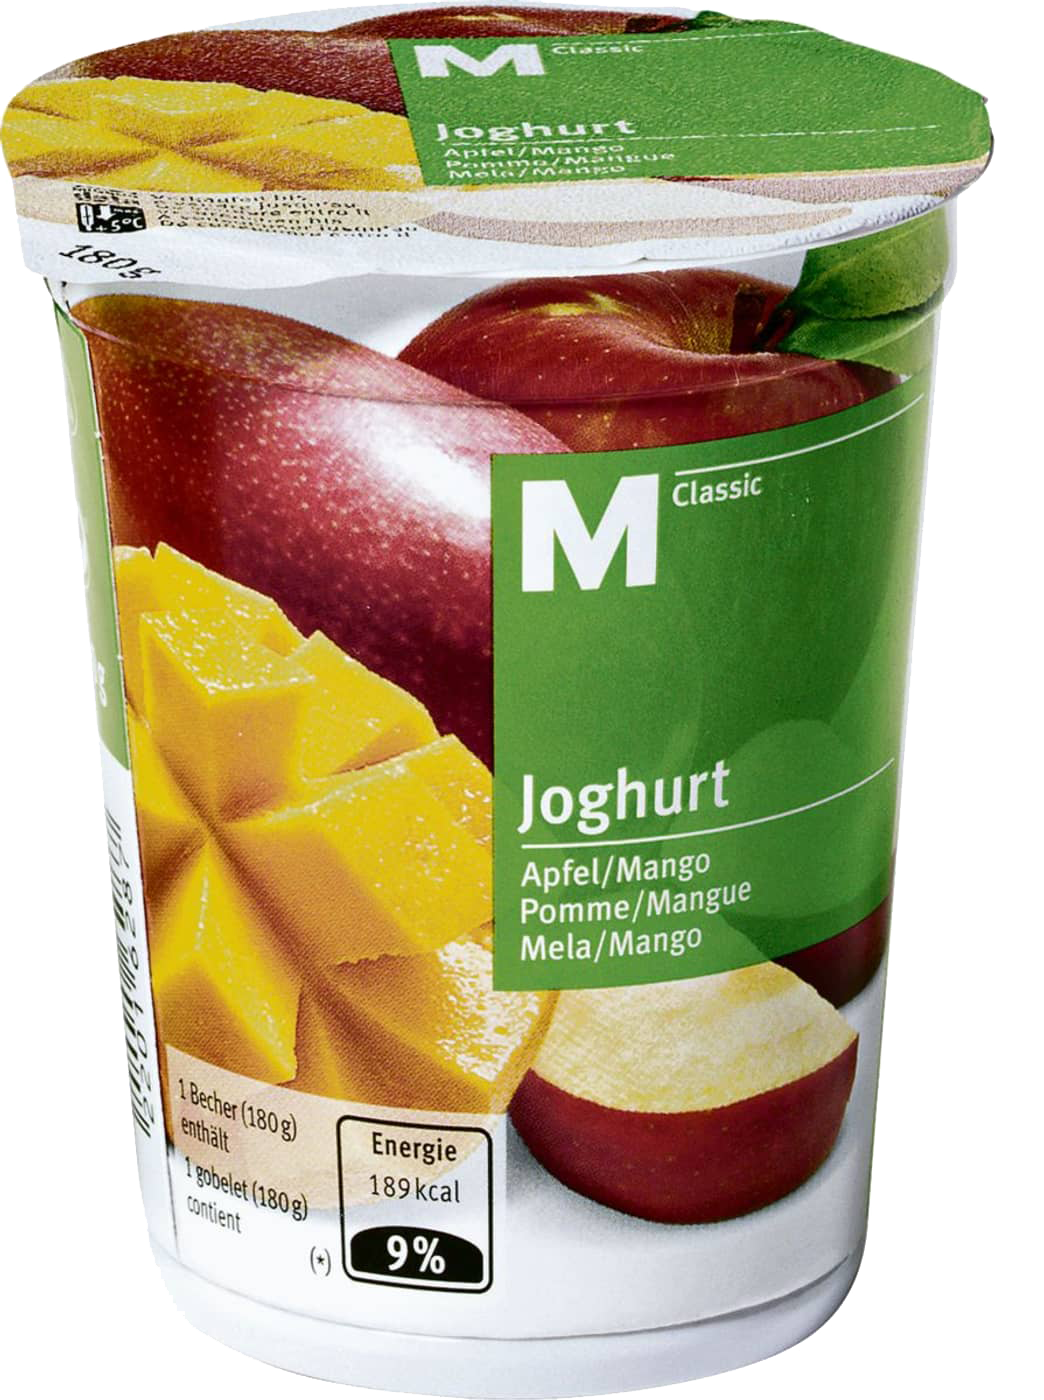
\includegraphics[height=2.5cm]{m-classic-joghurt-apfelmango} 
				\end{subfigure}$c_1$
				\begin{subfigure}{0.25\textwidth}
						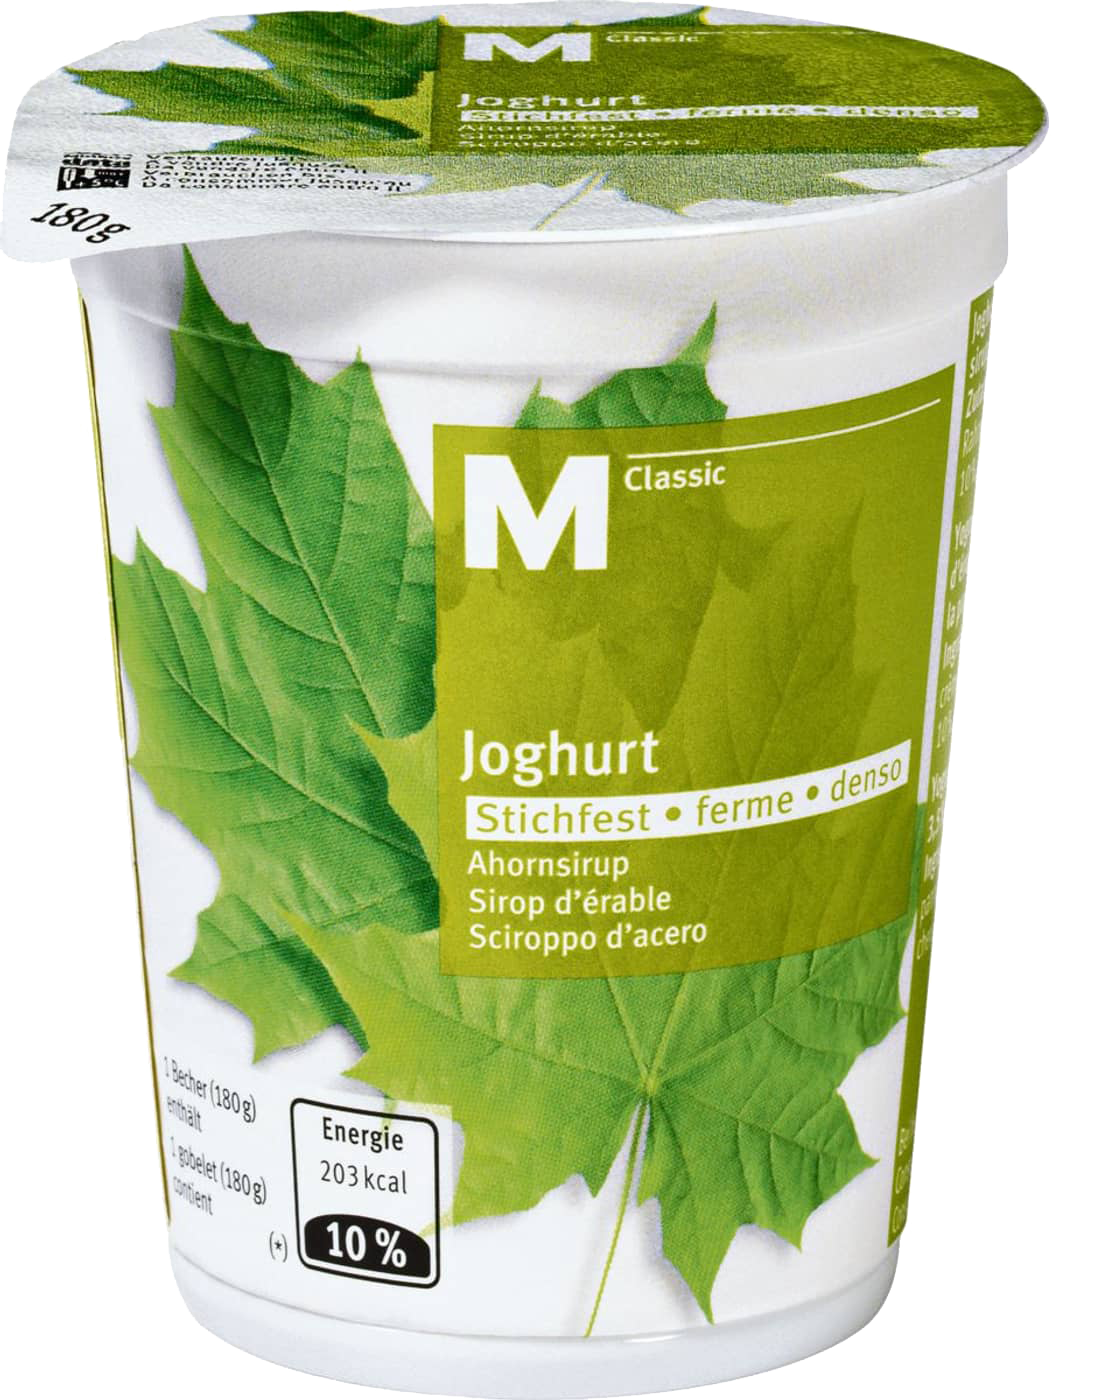
\includegraphics[height=2.5cm]{m-classic-joghurt-ahornsirup-stichfest} 
			\end{subfigure}	$c_2 \hdots$
		\end{subfigure}
	\end{figure}
\end{frame}



\begin{frame}{What is Uncertainty?}{What happens to these cases?}
\begin{figure}[H]
	\centering
	\begin{subfigure}{.32\textwidth}
		\centering
		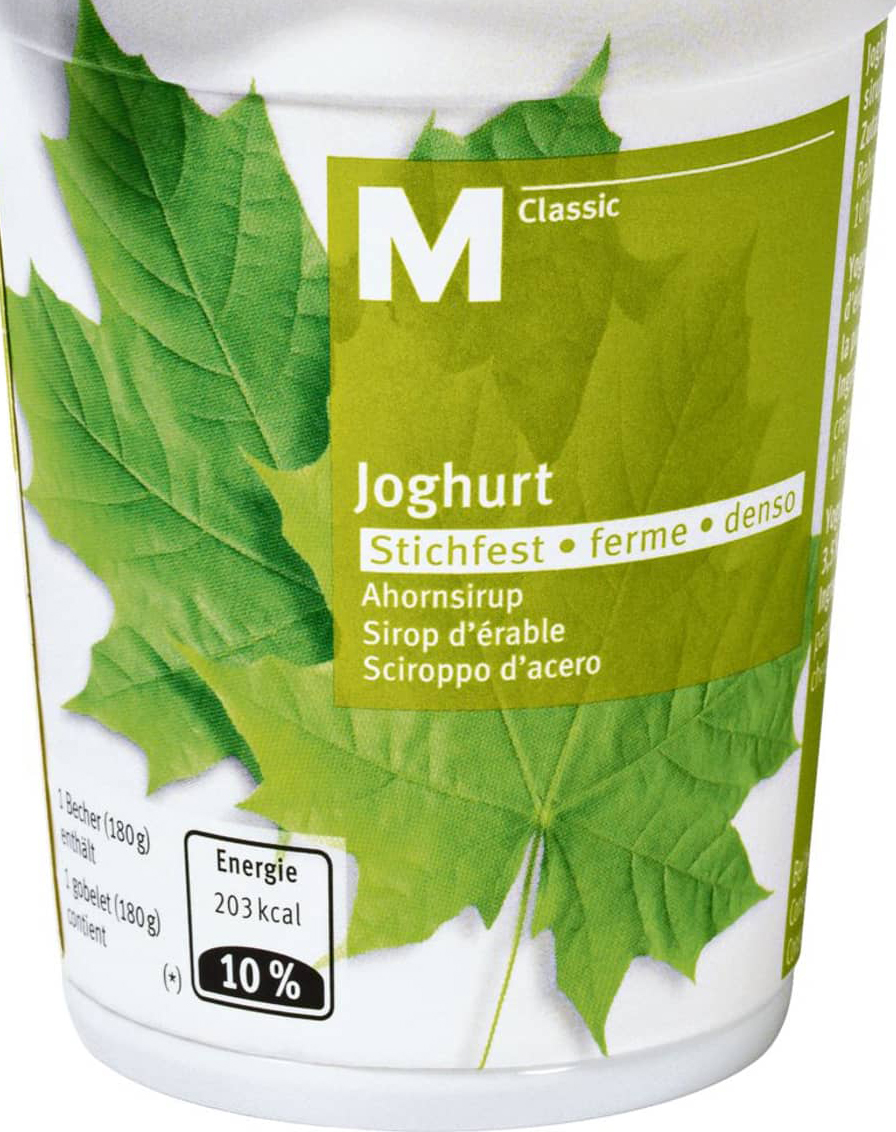
\includegraphics[width=\textwidth]{m-classic-joghurt-ahornsirup-stichfest-zoom1}
		\pause
		:)
	\end{subfigure}\pause
	\begin{subfigure}{.32\textwidth}
		\centering
		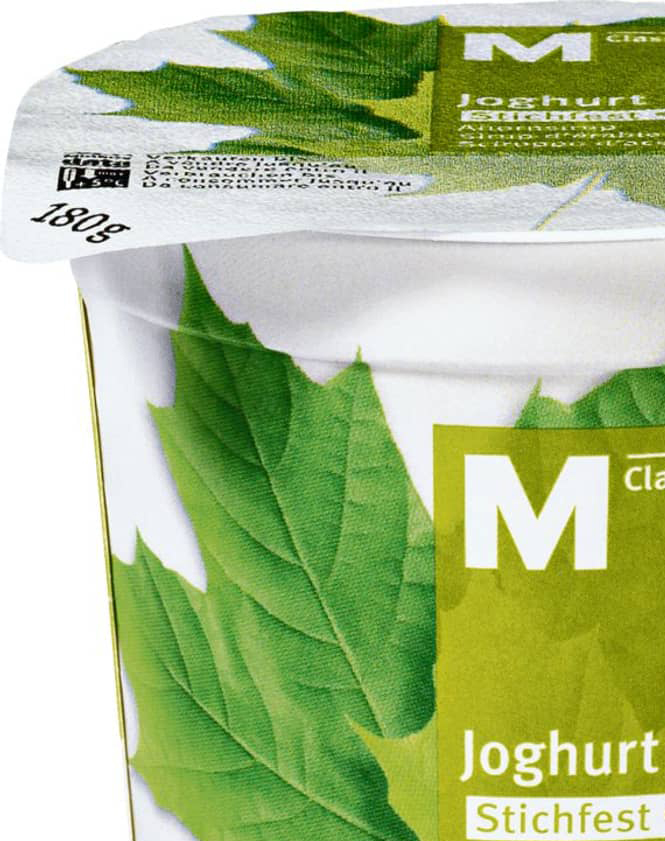
\includegraphics[width=\textwidth]{m-classic-joghurt-ahornsirup-stichfest-zoom2}
		\pause
		:)
	\end{subfigure}\pause
	\begin{subfigure}{.32\textwidth}
		\centering
		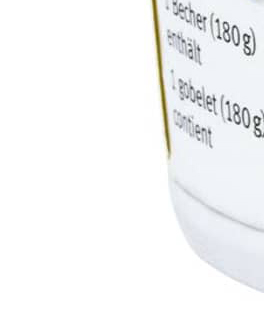
\includegraphics[width=\textwidth]{m-classic-joghurt-ahornsirup-stichfest-zoom3}
		\pause
		:(
	\end{subfigure}
\end{figure}
\end{frame}


% Novelty Detection
\begin{frame}{What is Uncertainty?}{What happens to this case?}
\begin{figure}[H]
	\centering
	\begin{subfigure}{0.22\textwidth}
		\centering
		Input image  of \textbf{unseen class} ``birchermüesli''\\[.5cm]
		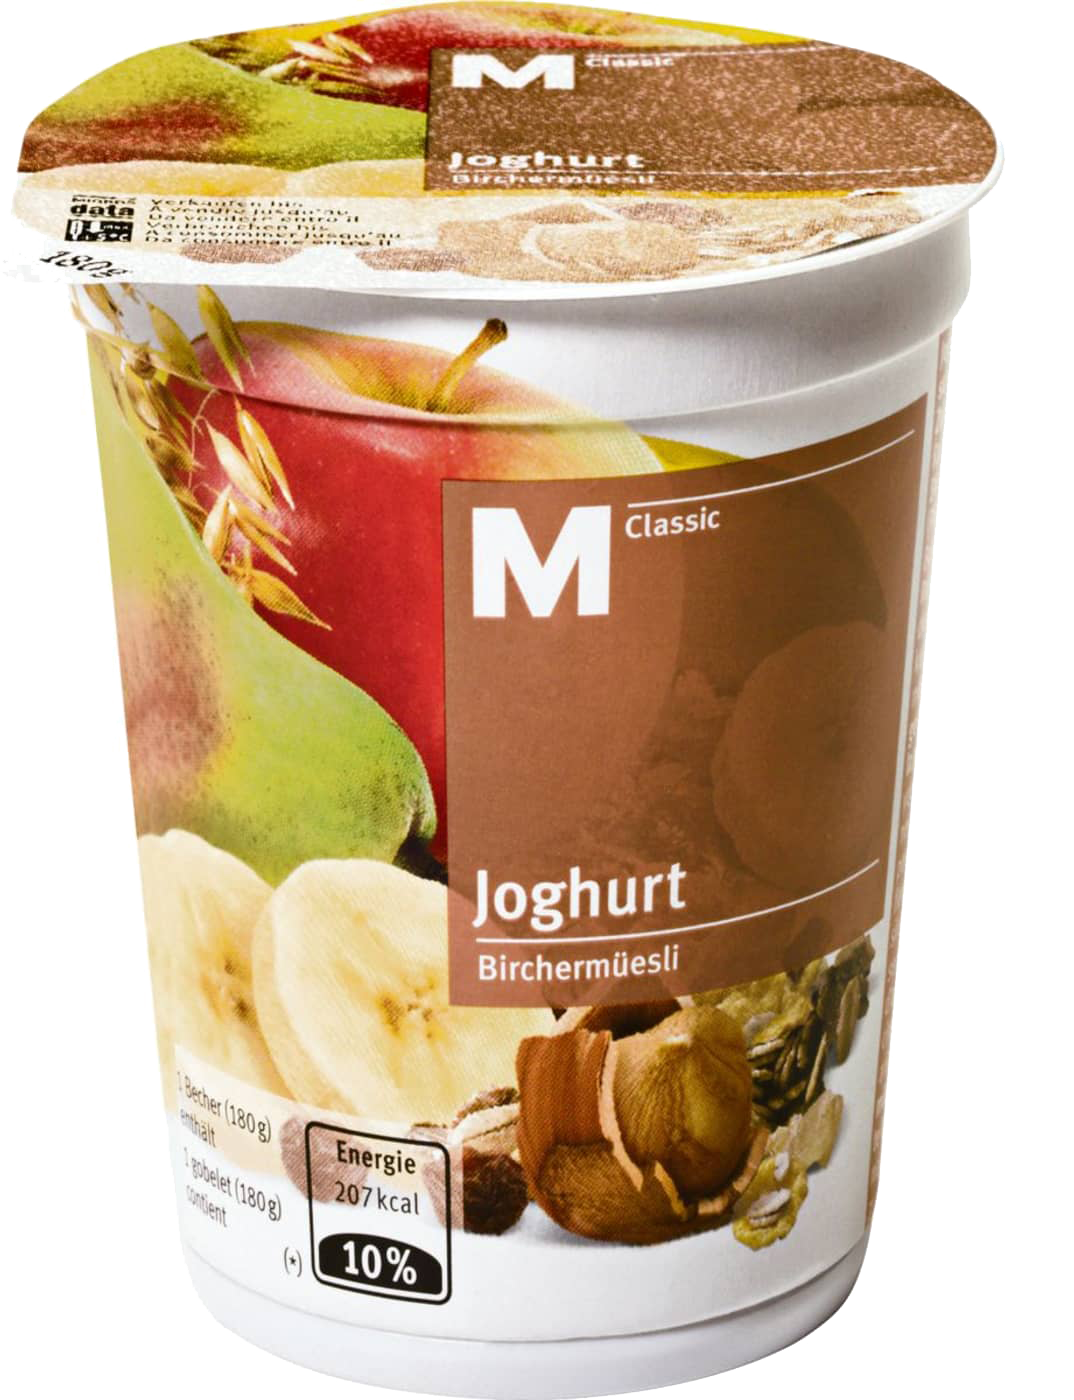
\includegraphics[height=2.5cm]{m-classic-joghurt-birchermueesli}
	\end{subfigure}$\Rightarrow$
	\begin{subfigure}{0.14\textwidth}
		\centering
		Model $M$
	\end{subfigure} $ \Rightarrow$
	\pause
	\begin{subfigure}{0.5\textwidth}
		\centering
		Set of classes:  $\mathcal{L}=\{c_1, c_2\}$\\ [.5cm]
		\begin{subfigure}{0.4\textwidth}
			\centering
			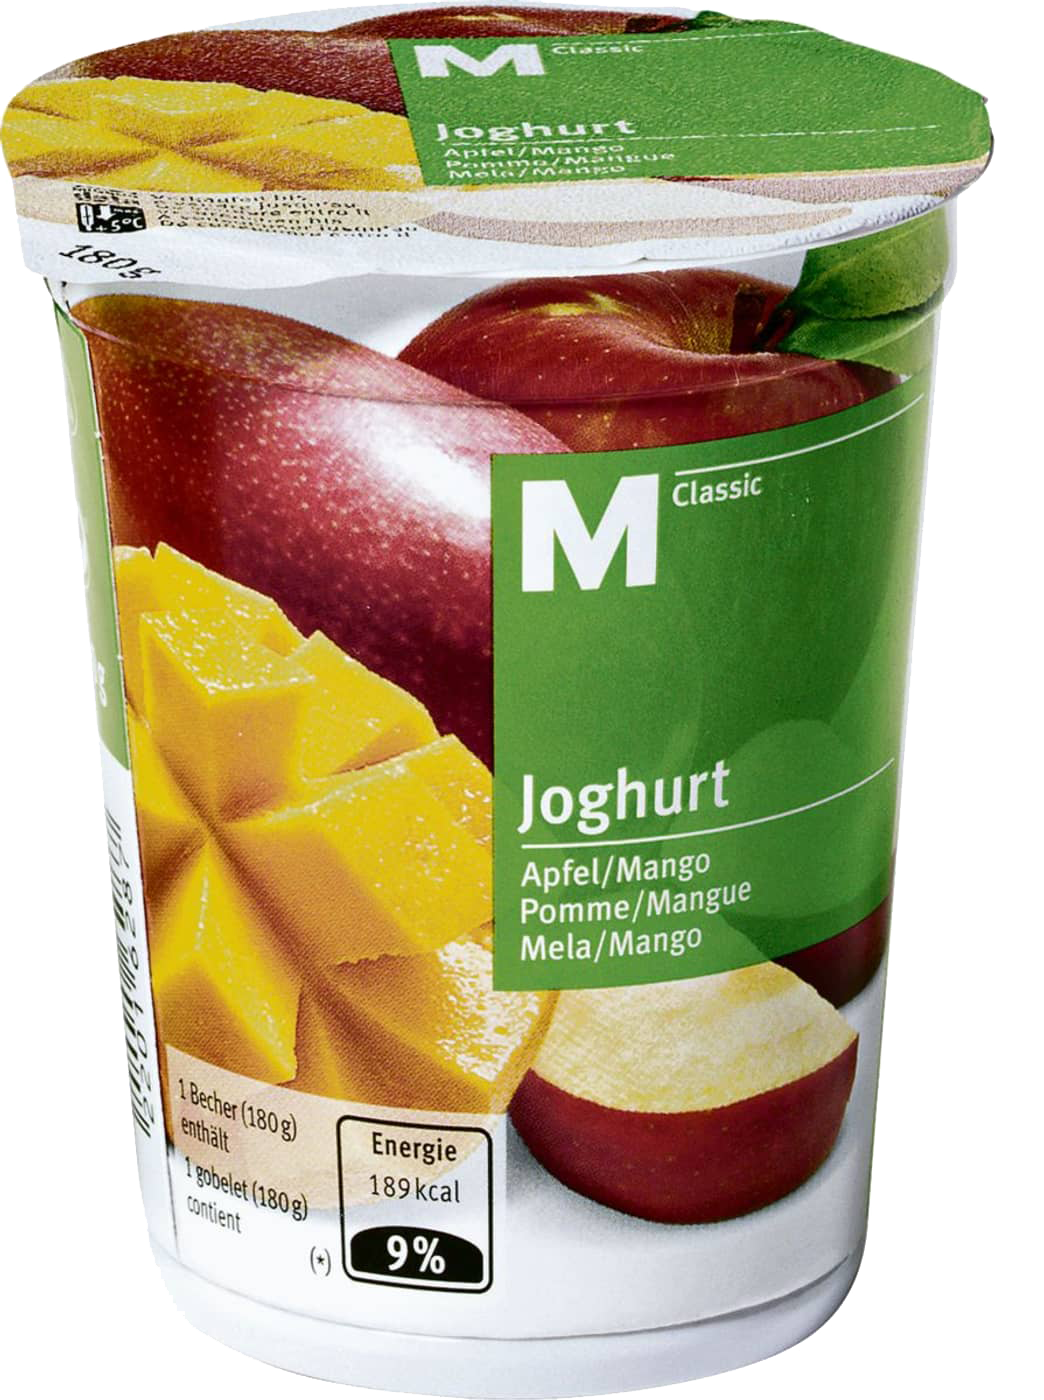
\includegraphics[height=2.5cm]{m-classic-joghurt-apfelmango}
			$p(c_1)=1$
		\end{subfigure}
		\begin{subfigure}{0.4\textwidth}
			\centering
			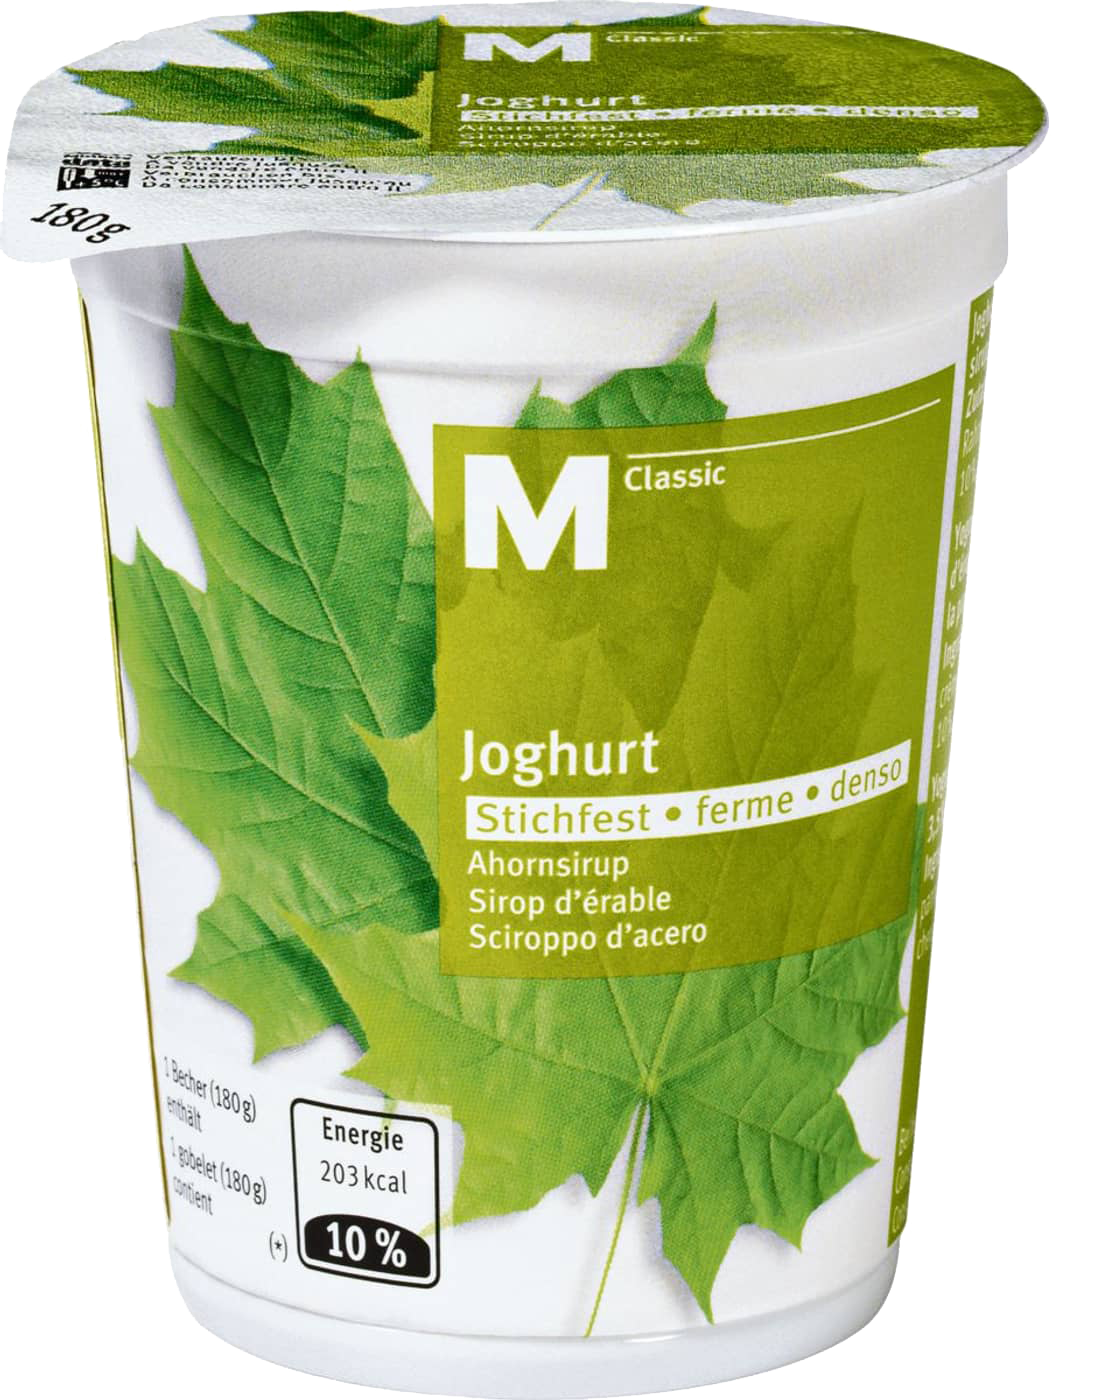
\includegraphics[height=2.5cm]{m-classic-joghurt-ahornsirup-stichfest} 
			$p(c_2)=0$
		\end{subfigure}
	\end{subfigure}
\end{figure}
\pause
\textbf{This is not what we want :(}
\end{frame}

% Novelty Detection
\begin{frame}{What is Uncertainty?}{What happens to this case?}
\begin{figure}[H]
\centering
\begin{subfigure}{0.22\textwidth}
	\centering
	Input image of \textbf{unseen class} ``birchermüesli''\\[.5cm]
	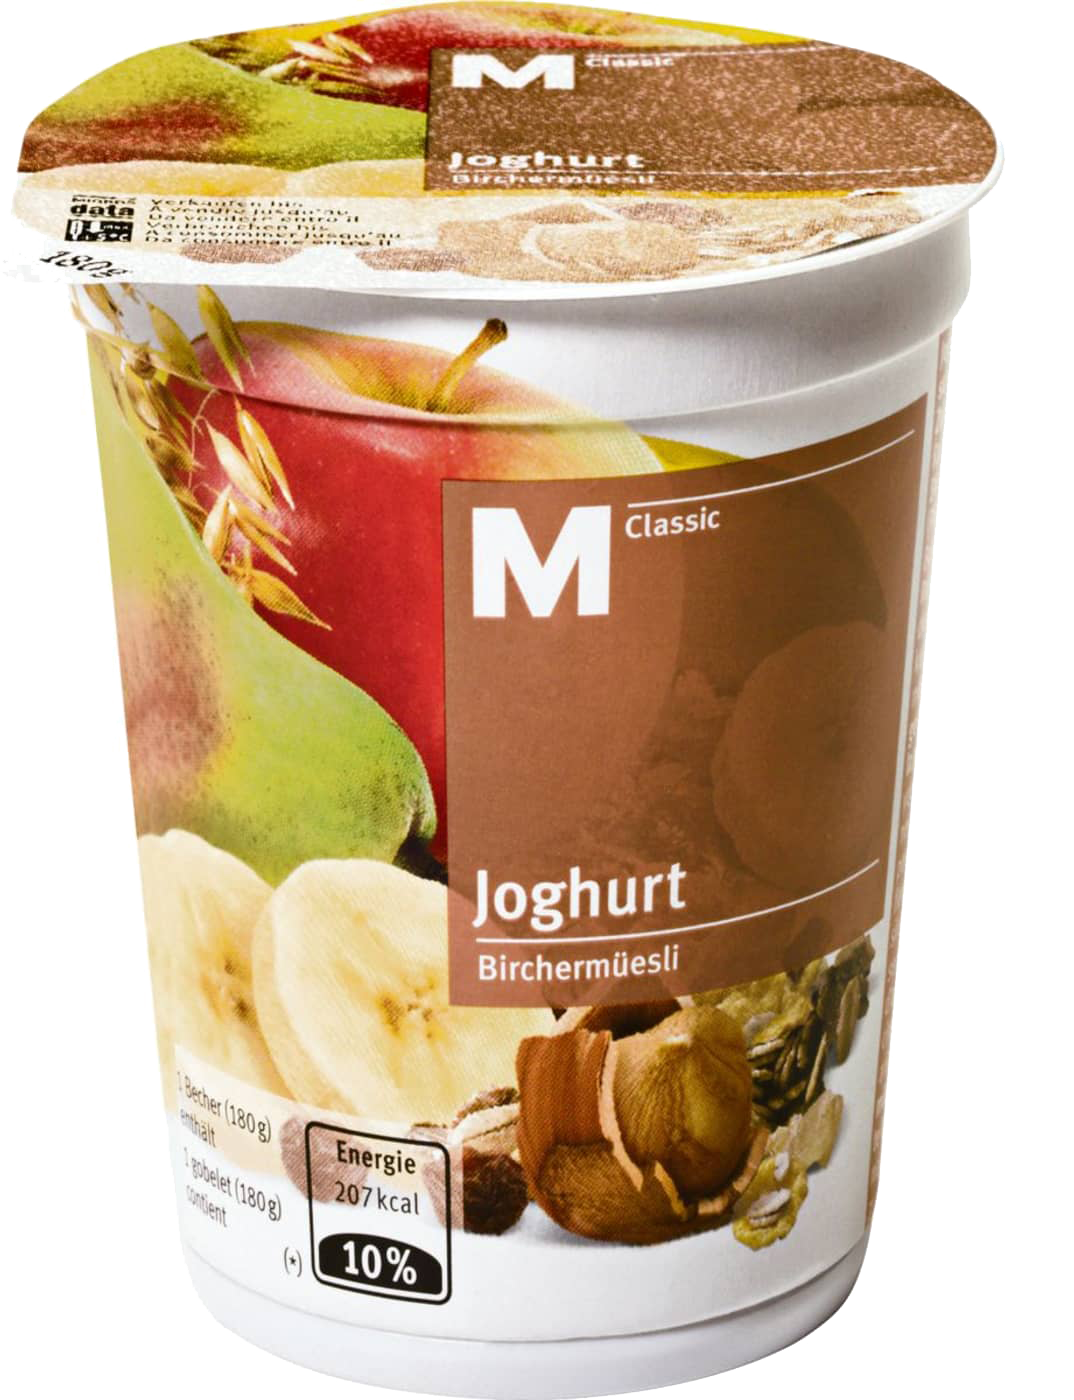
\includegraphics[height=2.5cm]{m-classic-joghurt-birchermueesli}
\end{subfigure}$\Rightarrow$
\begin{subfigure}{0.14\textwidth}
	\centering
	Model $M$
\end{subfigure} $ \Rightarrow$
\begin{subfigure}{0.5\textwidth}
	\centering
	Set of classes:  $\mathcal{L}=\{c_1, c_2\}$\\ [.5cm]
	\begin{subfigure}{0.4\textwidth}
		\centering
		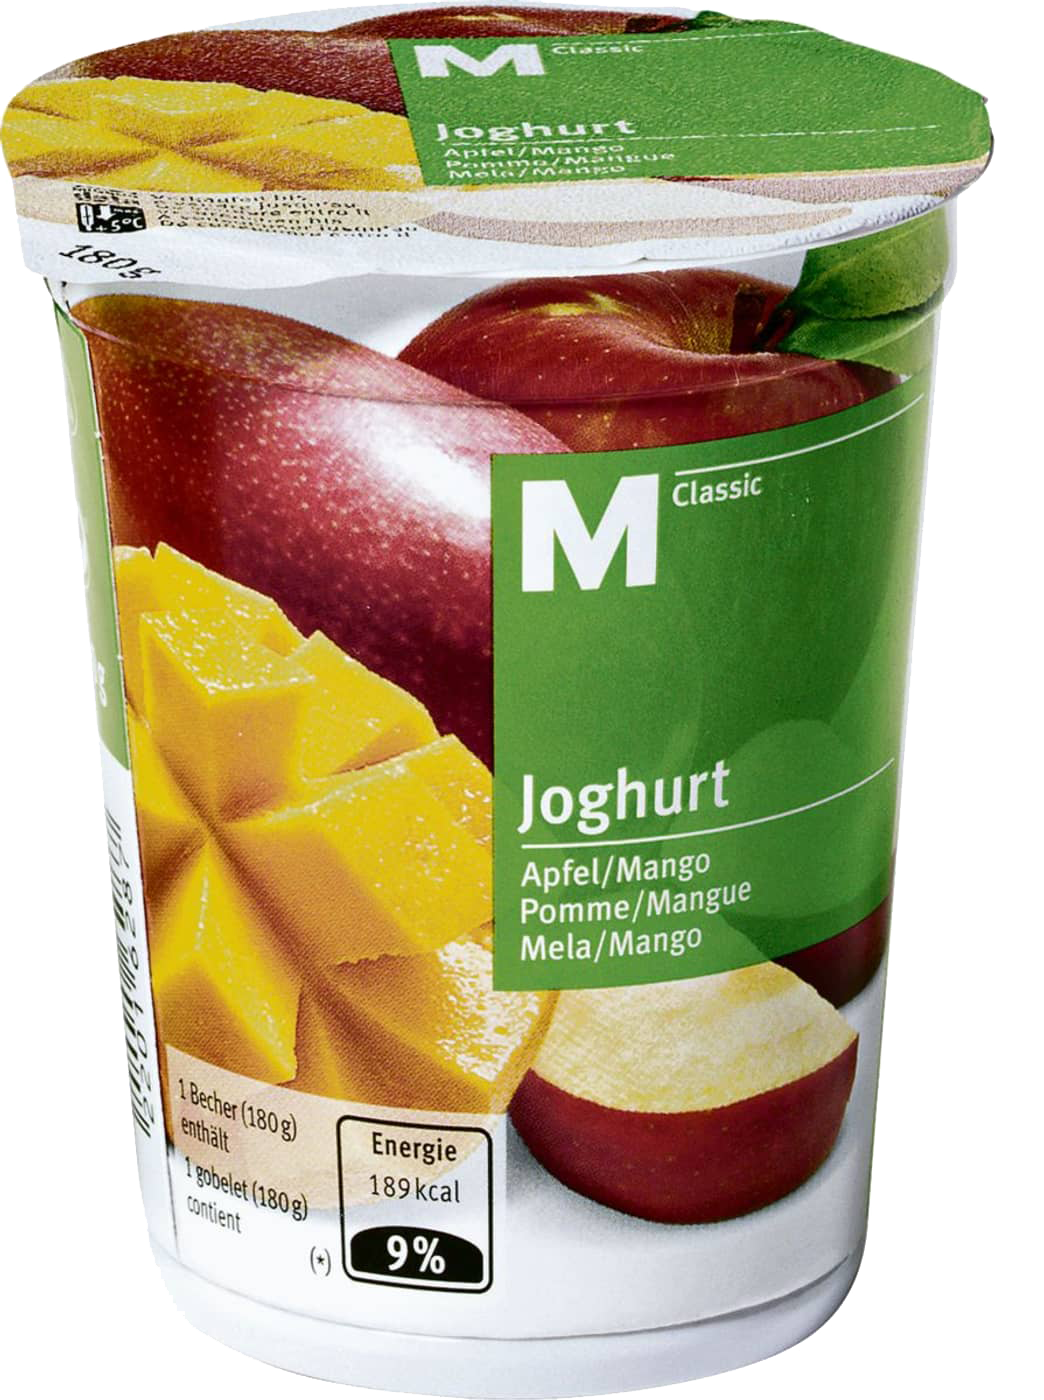
\includegraphics[height=2.5cm]{m-classic-joghurt-apfelmango}
		$p(c_1)=0.5$
	\end{subfigure}
	\begin{subfigure}{0.4\textwidth}
		\centering
		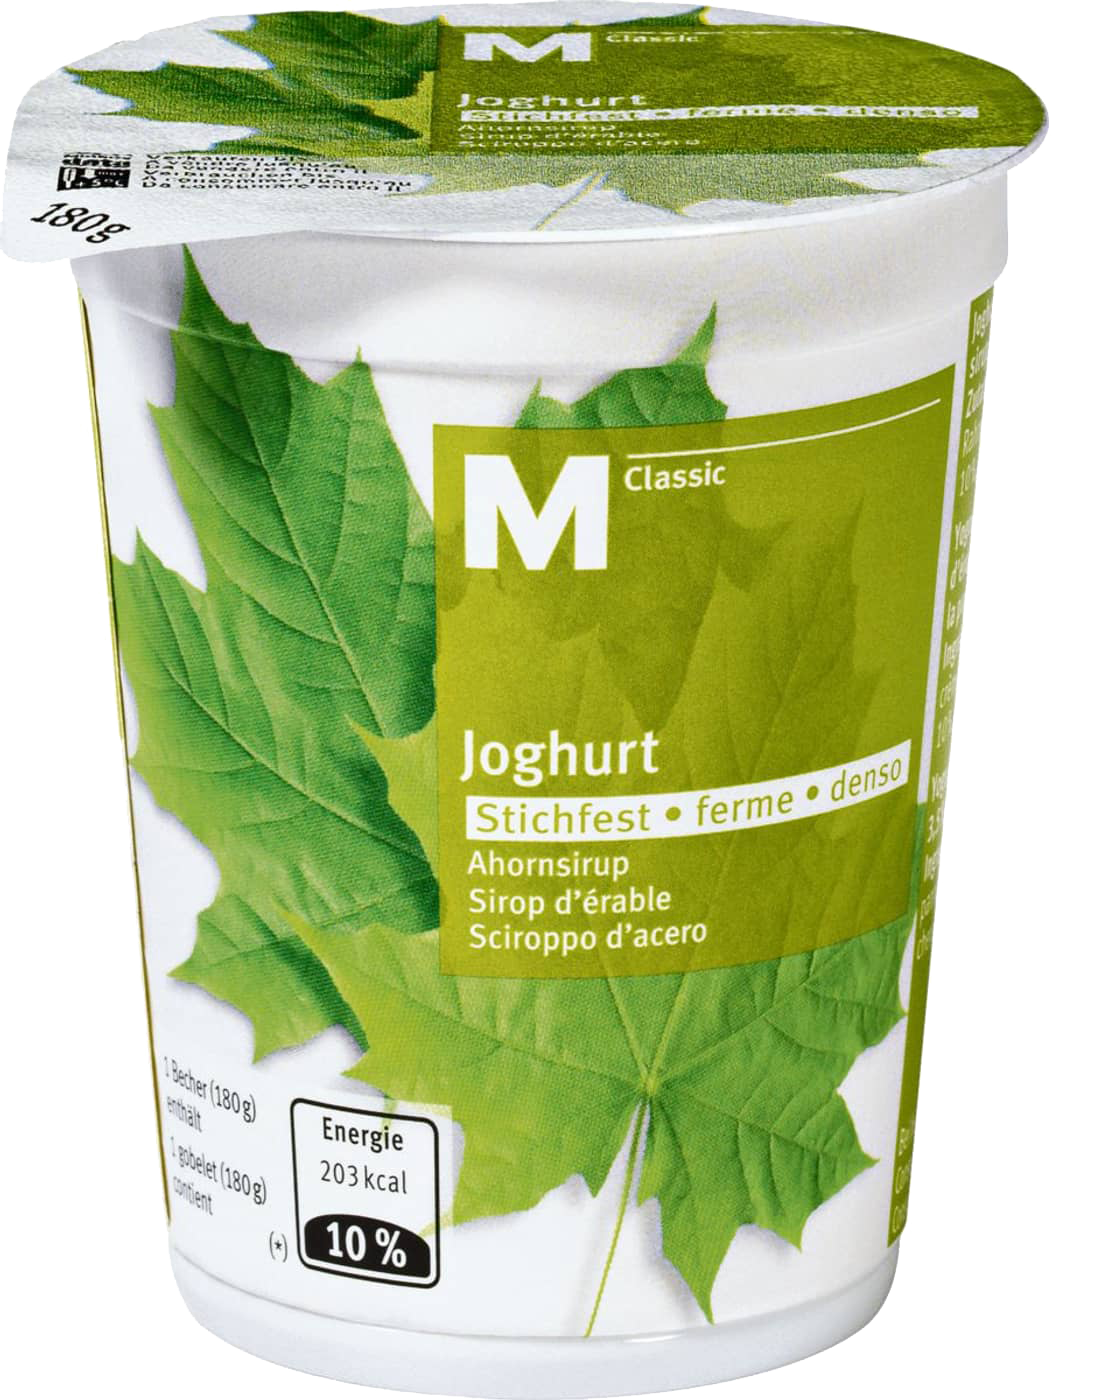
\includegraphics[height=2.5cm]{m-classic-joghurt-ahornsirup-stichfest} 
		$p(c_2)=0.5$
	\end{subfigure}
\end{subfigure}
\end{figure}
\textbf{This would be better :)}
\end{frame}


\begin{frame}{What is Uncertainty?}
Uncertainty
\begin{itemize}
	\item Information on \textit{confidence} of the model
	\item Ability to model incomplete information
\end{itemize}
Evaluation heuristics
\begin{itemize}
	\item Error detection: wrong prediction $\Rightarrow$ low confidence
	\item Novelty detection: unseen class $\Rightarrow$ low confidence
\end{itemize}
\end{frame}

% Applications of uncertainty
\begin{frame}{Relevant applications of Uncertainty}{Other than yoghurt classification}
\begin{figure}[H]
	\centering
	\begin{subfigure}{0.28\textwidth}
		\centering
		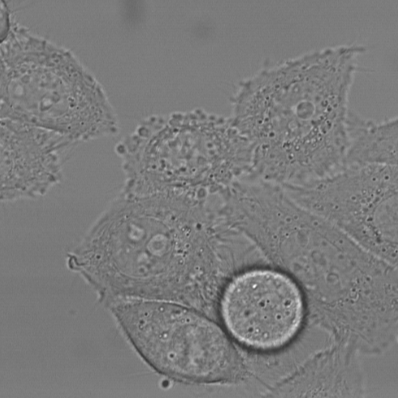
\includegraphics[width=\textwidth]{medical-imaging}	
		\caption{Medical imaging}
	\end{subfigure}
	\pause
	\begin{subfigure}{0.26\textwidth}	
		\centering
		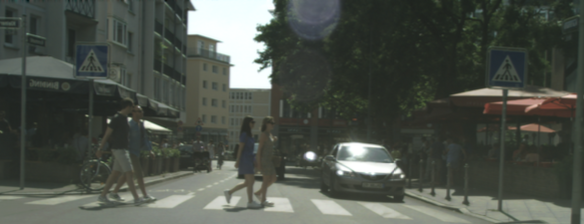
\includegraphics[width=\textwidth]{autonomous-driving-im}
		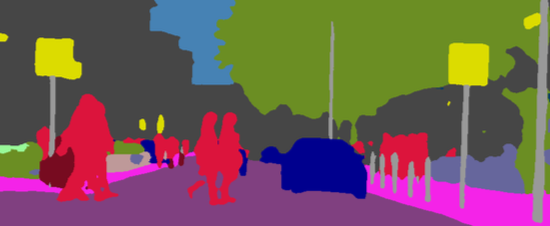
\includegraphics[width=\textwidth]{autonomous-driving-sem}\\[.2cm]
		
\includegraphics[width=.3\textwidth]{Tesla_Motors}\\
		\caption{Autonomous cars}
	\end{subfigure}
	\pause
	\begin{subfigure}{0.38\textwidth}
		\centering
		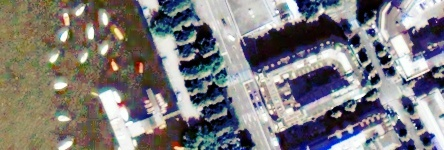
\includegraphics[width=\textwidth]{Im_11_detail.jpg}
		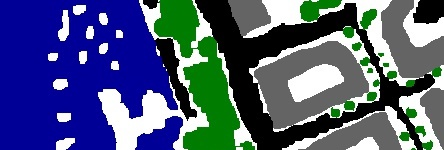
\includegraphics[width=\textwidth]{GT_11_detail.jpg}
		\caption{Land Cover Classification}
	\end{subfigure}
\end{figure}
\end{frame}

\subsection{How does Machine Learning work?}

\begin{frame}{How does Machine Learning work?}{Goals}
Terminology
\begin{itemize}
	\item \textbf{Image classification}: For a given image attribute one class label, i.e.:
	\begin{figure}[H]
		\begin{subfigure}{.1\textwidth}
			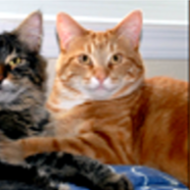
\includegraphics[width=\textwidth]{cat} 
		\end{subfigure} $\Rightarrow$ cat
		\begin{subfigure}{.1\textwidth}
			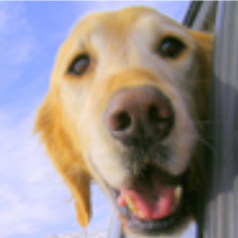
\includegraphics[width=\textwidth]{dog}
		\end{subfigure} $\Rightarrow$ dog
	\end{figure}
	\begin{figure}[H]
		\begin{subfigure}{.1\textwidth}
			
\includegraphics[width=\textwidth]{MNIST_cl_1_0} 
		\end{subfigure} $\Rightarrow$ ``1''
		\begin{subfigure}{.1\textwidth}
			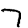
\includegraphics[width=\textwidth]{MNIST_cl_7_0}
		\end{subfigure} $\Rightarrow$ ``7''
	\end{figure}\pause
	\item \textbf{Semantic segmentation}: segmentation of an image into class labels
	\begin{figure}[H]
		\begin{subfigure}{0.38\textwidth}
			\centering
			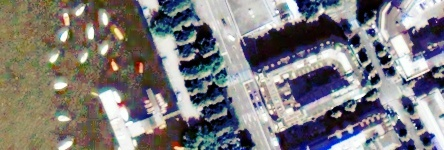
\includegraphics[width=\textwidth]{Im_11_detail.jpg}
		\end{subfigure} $\Rightarrow$
		\begin{subfigure}{0.38\textwidth}
			\centering
			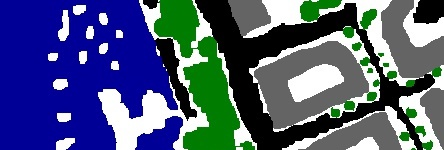
\includegraphics[width=\textwidth]{GT_11_detail.jpg}
		\end{subfigure}
	\end{figure}
\end{itemize}
\end{frame}


\begin{frame}{How does Machine Learning work?}
% MNIST images
	\begin{figure}[H]
		\begin{subfigure}{.7\textwidth}
			\centering
			\textbf{Training}\\[.2cm]
			% loop rows
			Dataset:\\
			\foreach \j in {0,...,2}
			{
				% loop classes
				\foreach \i in {0,...,9}
				{
					\begin{subfigure}{.07\textwidth}
						\centering
						\includegraphics[width=\textwidth]{MNIST_cl_\i_\j}
					\end{subfigure}
				}
				\\
			}
			$\vdots$\\[.2cm]
			Labels: 0, 1, 2, 3, 4, 5, 6, 7, 8, 9\\[.2cm]
			$\Downarrow$\\[.2cm]
			Training (+ Validation)\\[.2cm]
			$\Downarrow$\\[.2cm]
			Model $M$
		\end{subfigure}\pause
		\begin{subfigure}{.28\textwidth}
			\centering
			\textbf{Prediction}\\[.2cm]
			New image:\\[.2cm]
			
\includegraphics[width=.2\textwidth]{MNIST_cl_1_1}\\[.2cm]
			$\Downarrow$\\[.2cm]
			Prediction using model $M$\\[.2cm]
			$\Downarrow$\\[.2cm]
			Label: 1
		\end{subfigure}
		\label{fig:MNIST-Im}
	\end{figure}
\end{frame}

\begin{frame}{How does Machine Learning work?}{\glspl{CNN}}
	\begin{figure}[H]
		\centering
		\only<1>{
			\begin{subfigure}{.65\textwidth}
				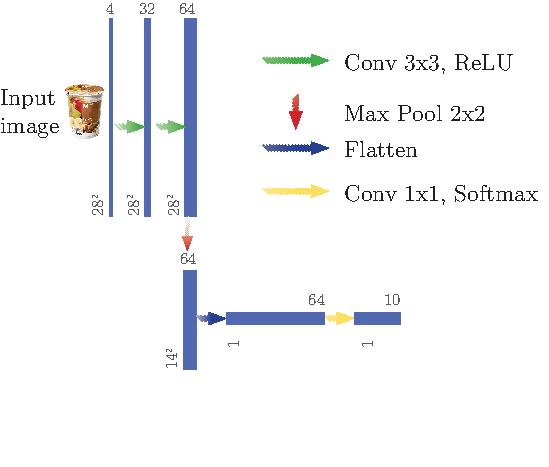
\includegraphics[width=\textwidth]{mnist}
			\end{subfigure}
			\hfill
		}
		\only<2>{
			\begin{subfigure}{.65\textwidth}
				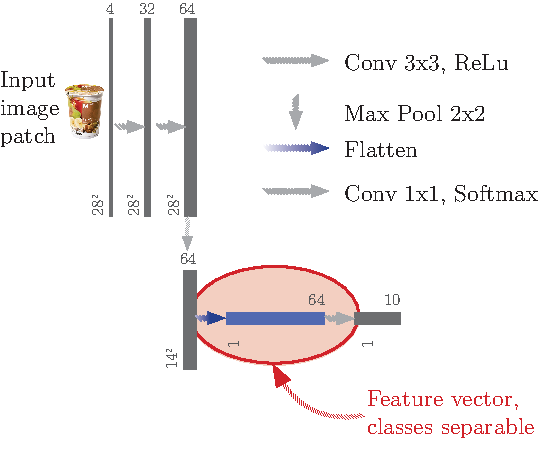
\includegraphics[width=\textwidth]{mnist_pre_softmax}
			\end{subfigure}
			\hfill
		}
		\only<3>{
			\begin{subfigure}{.65\textwidth}
				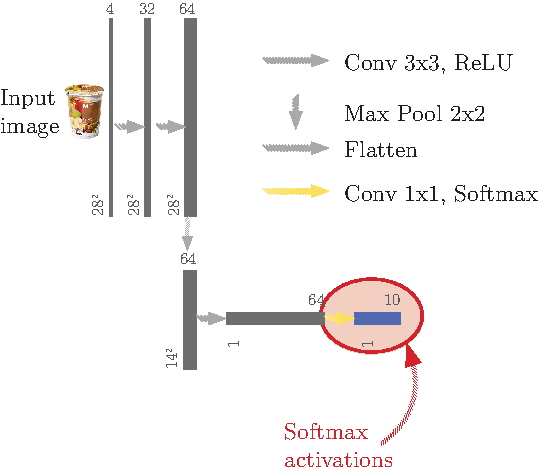
\includegraphics[width=\textwidth]{mnist_softmax}
			\end{subfigure}\hfill
		\begin{subfigure}{.28\textwidth}
			\begin{tabular}{cc}
				\toprule
				p(\raisebox{-.35cm}{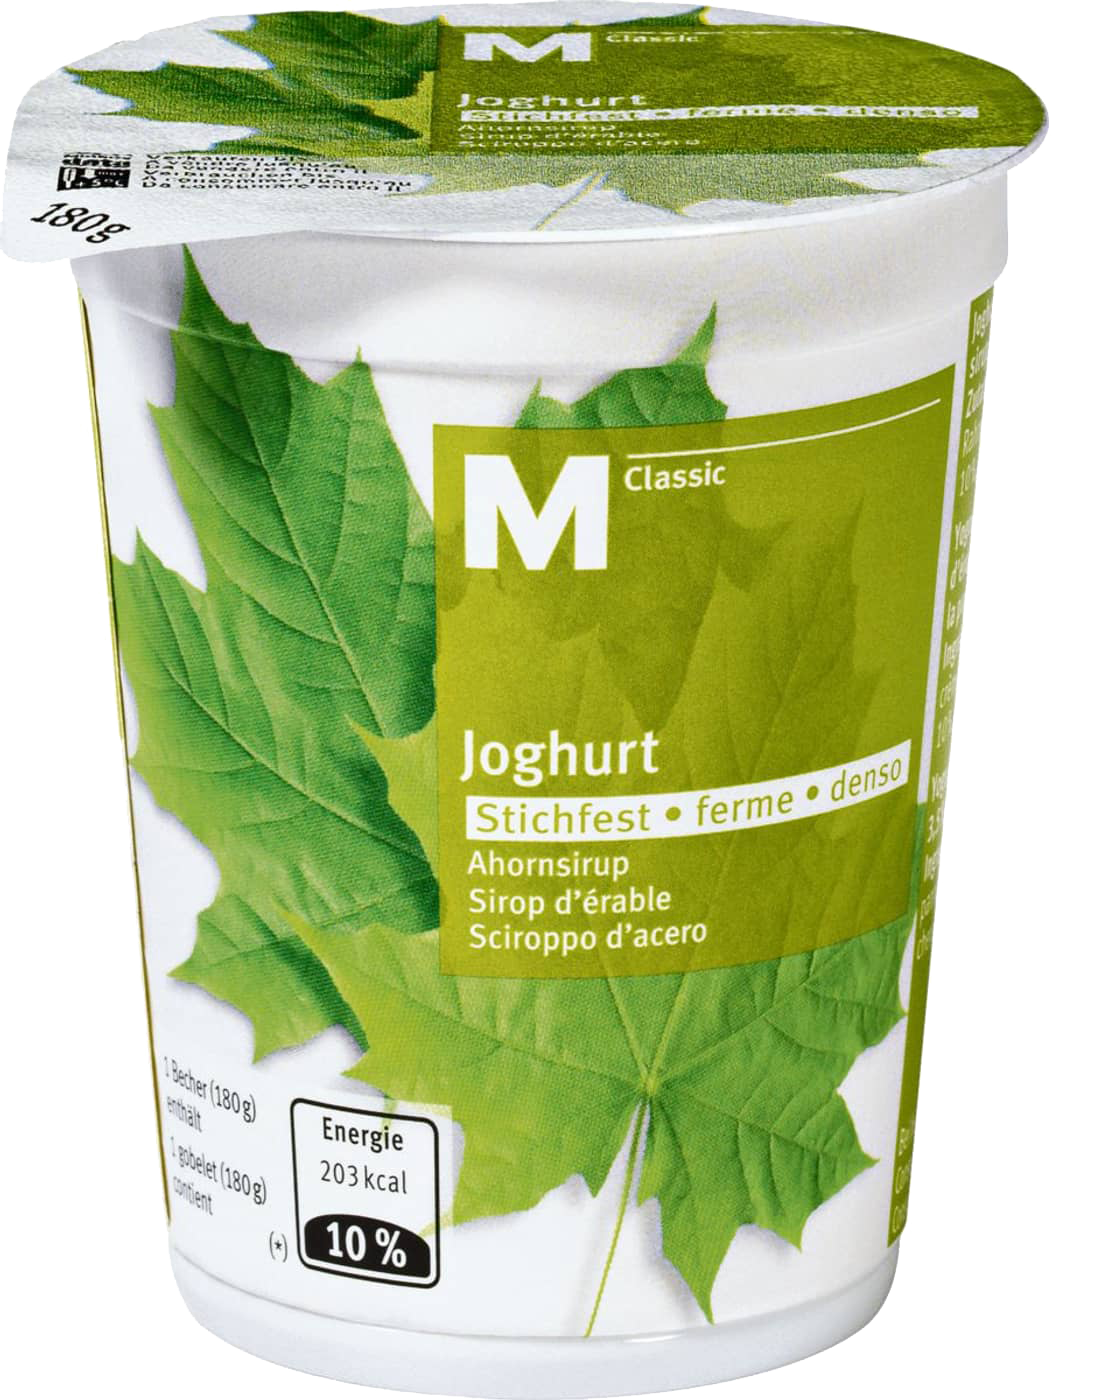
\includegraphics[width=.7cm]{m-classic-joghurt-ahornsirup-stichfest}})=& .3  \\ 
				p(\raisebox{-.35cm}{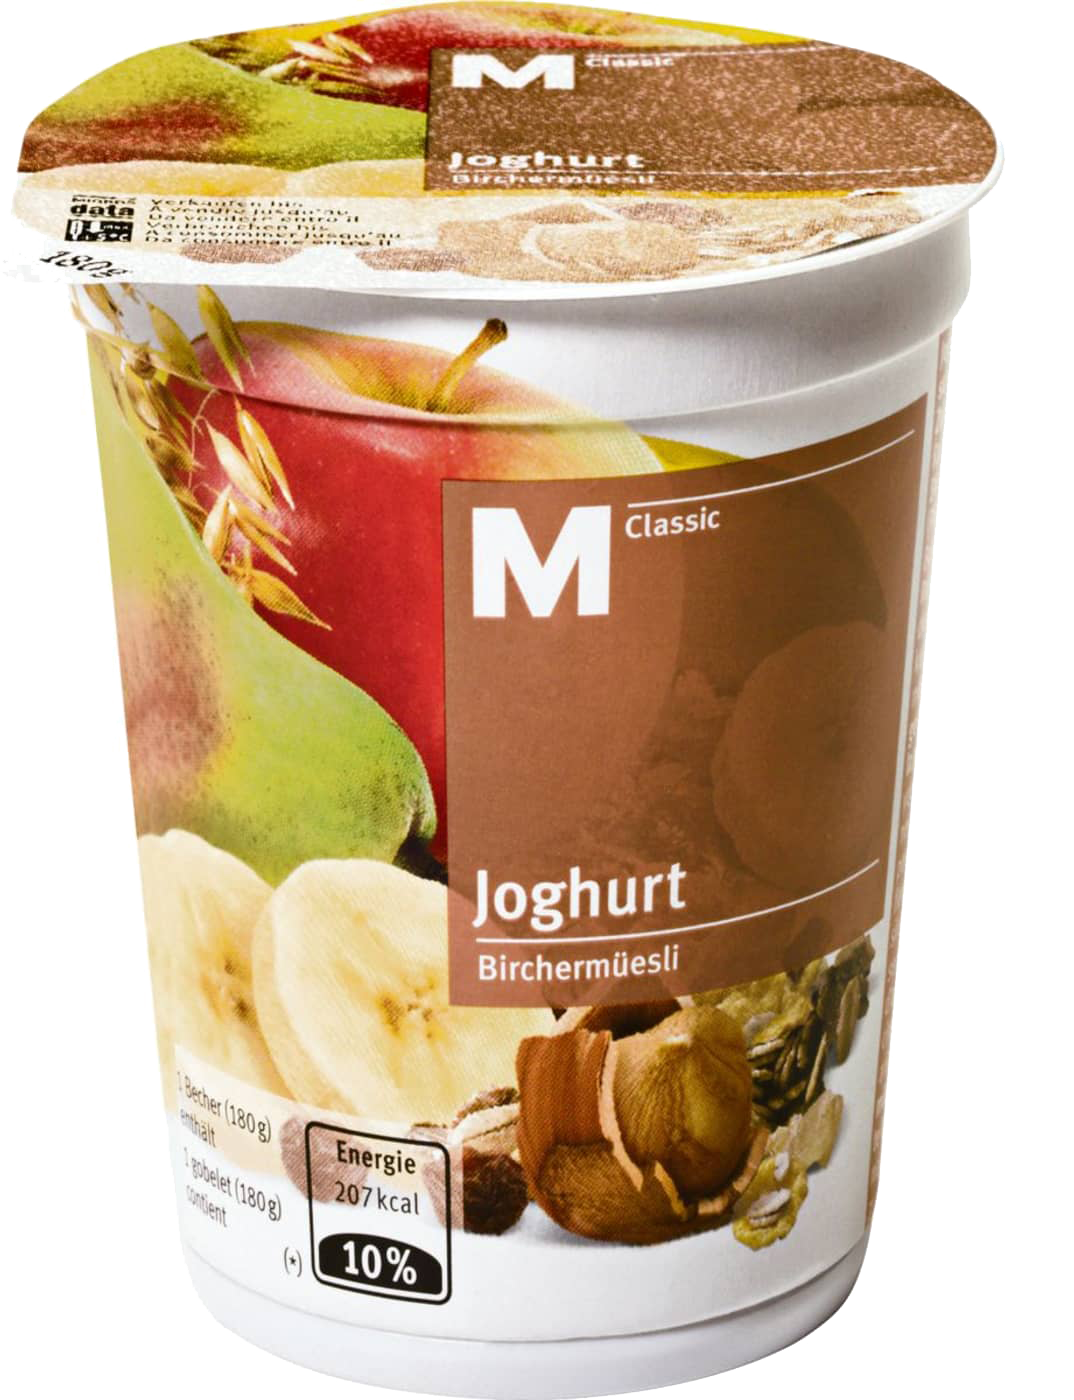
\includegraphics[width=.7cm]{m-classic-joghurt-birchermueesli}})=& \textbf{.4}  \\
				p(\raisebox{-.35cm}{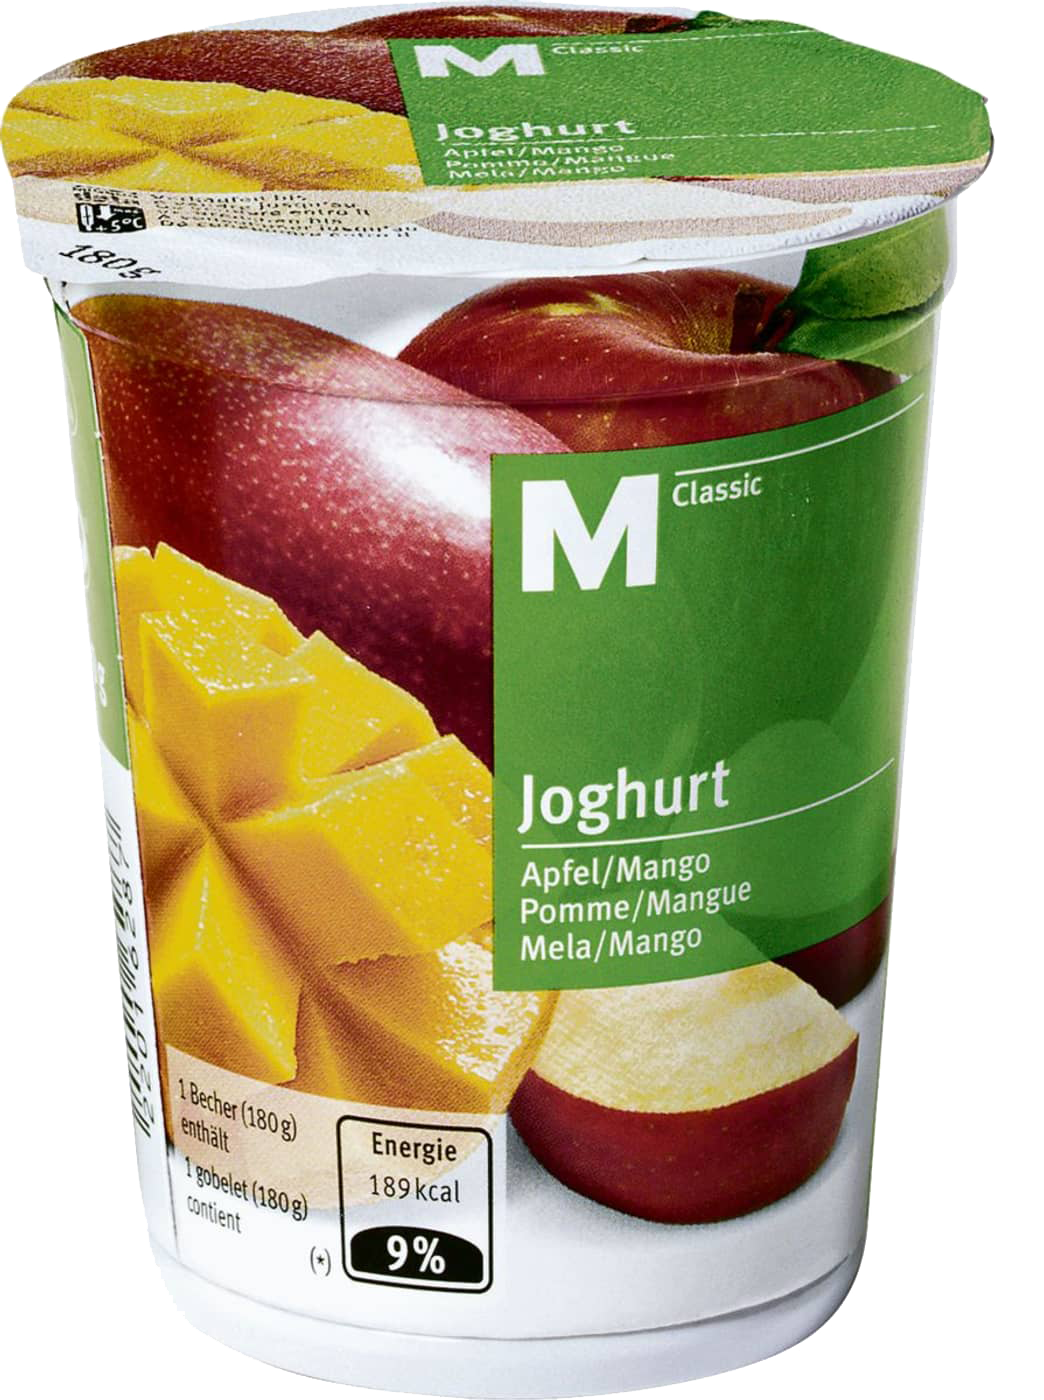
\includegraphics[width=.7cm]{m-classic-joghurt-apfelmango}})=& .3  \\ \midrule
				Sum & 1  \\ \bottomrule
			\end{tabular}\hfill
		\end{subfigure}
		}
	\end{figure}
\end{frame}


\begin{frame}{Research objectives}
	\begin{itemize}
		\item Determine uncertainty of standard \glspl{CNN} using
		\begin{itemize}
			\item softmax-based methods
			\item methods based on pre-softmax activations
		\end{itemize}
		\item In particular, implement \acrlongpl{DF} and compare them to baseline methods
		\item Evaluate these uncertainty measures in terms of their performance for \textbf{novelty detection}
	\end{itemize}
\end{frame}

\section{Methodology}
\subsection{Literature Review}

\begin{frame}{Types of Uncertainty Measures}
	\begin{enumerate}
	\item Based on new network architectures
	\item \textit{Using standard network architectures}
	\begin{itemize}
		\item Based on network output (i.e., softmax activations)
		\item Using network activations before the final classification layer
	\end{itemize}
	\end{enumerate}
\end{frame}


\begin{frame}{Uncertainty based on Network Output}{Problems}
Problems with softmax output
\begin{itemize}
	\item Can be easily fooled
	\begin{figure}[H]
		\centering
		\begin{subfigure}{.1\textwidth}
			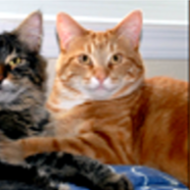
\includegraphics[width=\textwidth]{cat} 
		\end{subfigure} $\Rightarrow$ cat\hspace{1cm}
		\begin{subfigure}{.1\textwidth}
			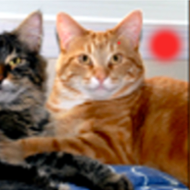
\includegraphics[width=\textwidth]{cat_fooled}
		\end{subfigure} $\Rightarrow$ dog
	\end{figure}
	\item Not robust to minor transformations
	\begin{figure}[H]
		\centering
		\begin{subfigure}{.1\textwidth}
			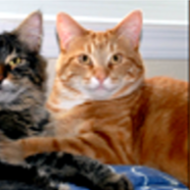
\includegraphics[width=\textwidth]{cat} 
		\end{subfigure} $\Rightarrow$ cat \hspace{1cm}
		\begin{subfigure}{.1\textwidth}
			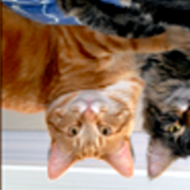
\includegraphics[width=\textwidth]{cat_notrobust}
		\end{subfigure} $\Rightarrow$ dog
	\end{figure}
	\item Can yield high scores despite being wrong
\end{itemize}
\end{frame}

\begin{frame}{Uncertainty based on Network Activations}
\begin{figure}[H]
	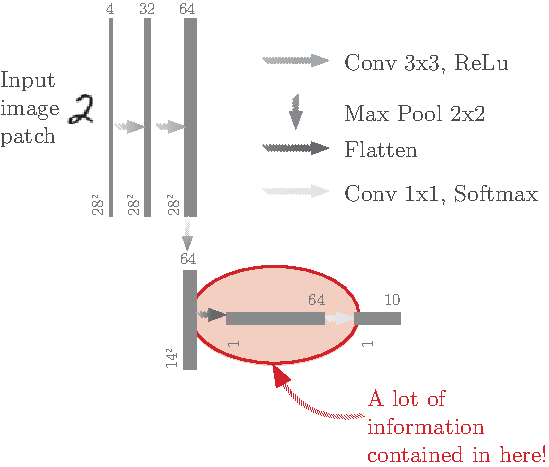
\includegraphics[width=.7\textwidth]{mnist_2}
\end{figure}
\end{frame}

%\begin{frame}{Uncertainty based on Network Output}
%	\vspace{-20pt}
%	\begin{block}{\textbf{\gls{MSR}}}   
%	\begin{equation*}
%	\label{eq:net_msr}
%	C_1(\mathbf{x})=P^{(c_1)}(\mathbf{x})
%	\end{equation*}
%	where $\mathbf{x}$ is a data point and $c_1=\argmax_{c\in\mathcal{L}}P^{(c)}(\mathbf{x})$.
%	\end{block}
%	
%	\begin{block}{\textbf{Margin}}   
%	\begin{equation*}
%	\label{eq:net_margin}
%	C(\mathbf{x})=P^{(c_1)}(\mathbf{x})-P^{(c_2)}(\mathbf{x})
%	\end{equation*}
%	where $c_1=\argmax_{c\in\mathcal{L}}P^{(c)}(\mathbf{x})$ and $c_2=\argmax_{c\in\mathcal{L}\setminus c_1}P^{(c)}(\mathbf{x})$.
%	\end{block}
%	\begin{block}{\textbf{Entropy}}   
%	\begin{equation*}
%	\label{eq:net_entropy}
%	C_2(\mathbf{x}) = -H(\mathbf{P(\mathbf{x})}) = -\sum_{c\in \mathcal{L}}^{}P^{(c)}(\mathbf{x})\log P^{(c)}(\mathbf{x})
%	\end{equation*}
%	\end{block}
%\end{frame}


\begin{frame}{Uncertainty based on Network Output}

\begin{block}{Based on softmax activations}
\begin{itemize}
	\item \gls{MSR}
	\item Margin
	\item Entropy
\end{itemize}	
\end{block}

\begin{block}{\textbf{\gls{MC-Dropout}}}
	\begin{enumerate}
		\item Perform prediction \textit{using dropout}
		\item Repeat prediction $n$ times
		\item Prediction = mean of outputs, Certainty = variance of outputs
	\end{enumerate}
	$\Rightarrow$ Simplified version used:
	\begin{itemize}
		\item Dropout only in last layer before softmax
		\item Using entropy of mean output rather than variance
	\end{itemize}
\end{block}
\end{frame}


\begin{frame}{Novelty Detection Methods}
Goal: find samples belonging to novel, unseen classes
\begin{itemize}
	\item Model distribution or support of ``normal class''
	\item Attribute low confidence to samples of ``abnormal class''
\end{itemize}
$\Rightarrow$ Binary classification task!
\begin{block}{\glspl{GMM}}
\begin{itemize}
	\item Fit $n$ Gaussians to training data using \gls{EM}
	\item Predict log-likelihood of test data given the fitted distributions
\end{itemize}
\end{block}
\begin{block}{\glspl{OC-SVM}}
	\begin{itemize}
		\item Find support of the ``normal data'' class
		\item Use decision function to decide whether a data point is an inlier or outlier
	\end{itemize}
\end{block}
\end{frame}



\subsection{\acrlongpl{DF}}
\begin{frame}{Random Forests}{Idea}
Why should we need to model the ``normal class'' perfectly if we can do simpler?
\begin{itemize}
	\item Train many imperfect models (in parallel)
	\item Average them
\end{itemize}
\end{frame}
\begin{frame}{Random Forests}{A yoghurt example}
\begin{figure}
	\centering
	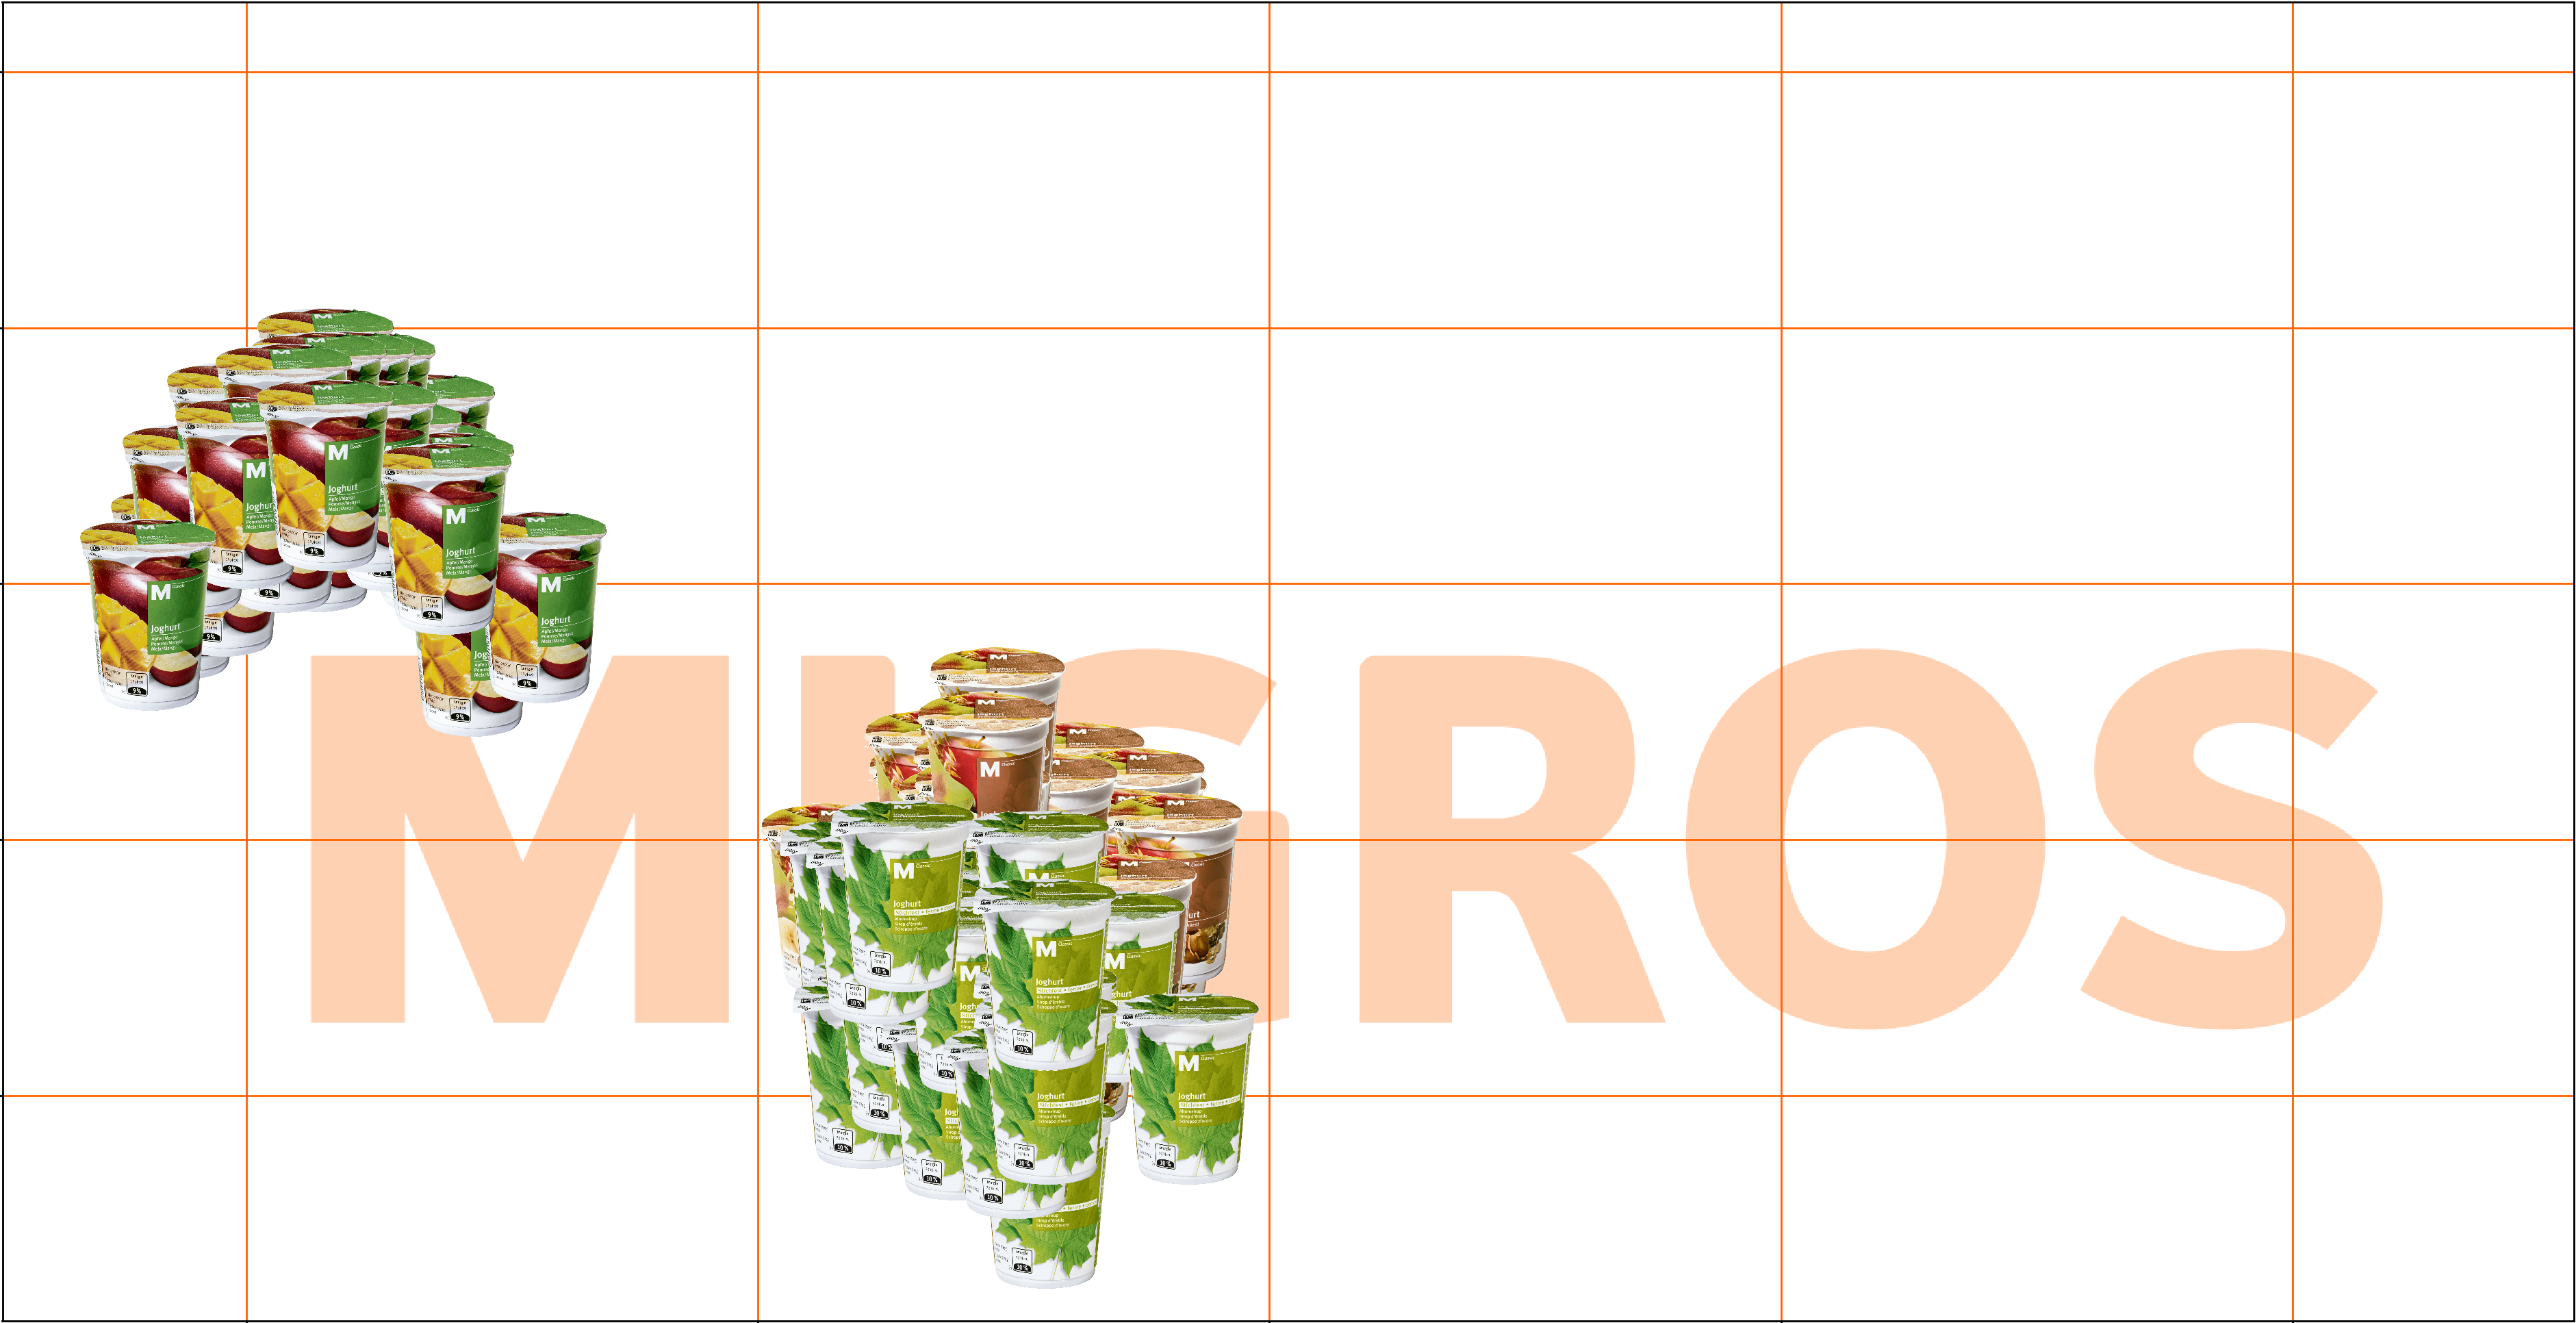
\includegraphics[width=\textwidth]{labelled-data-migros}
\end{figure}
\end{frame}

\begin{frame}{Random Forests}{A yoghurt example}
	\begin{figure}
		\centering
		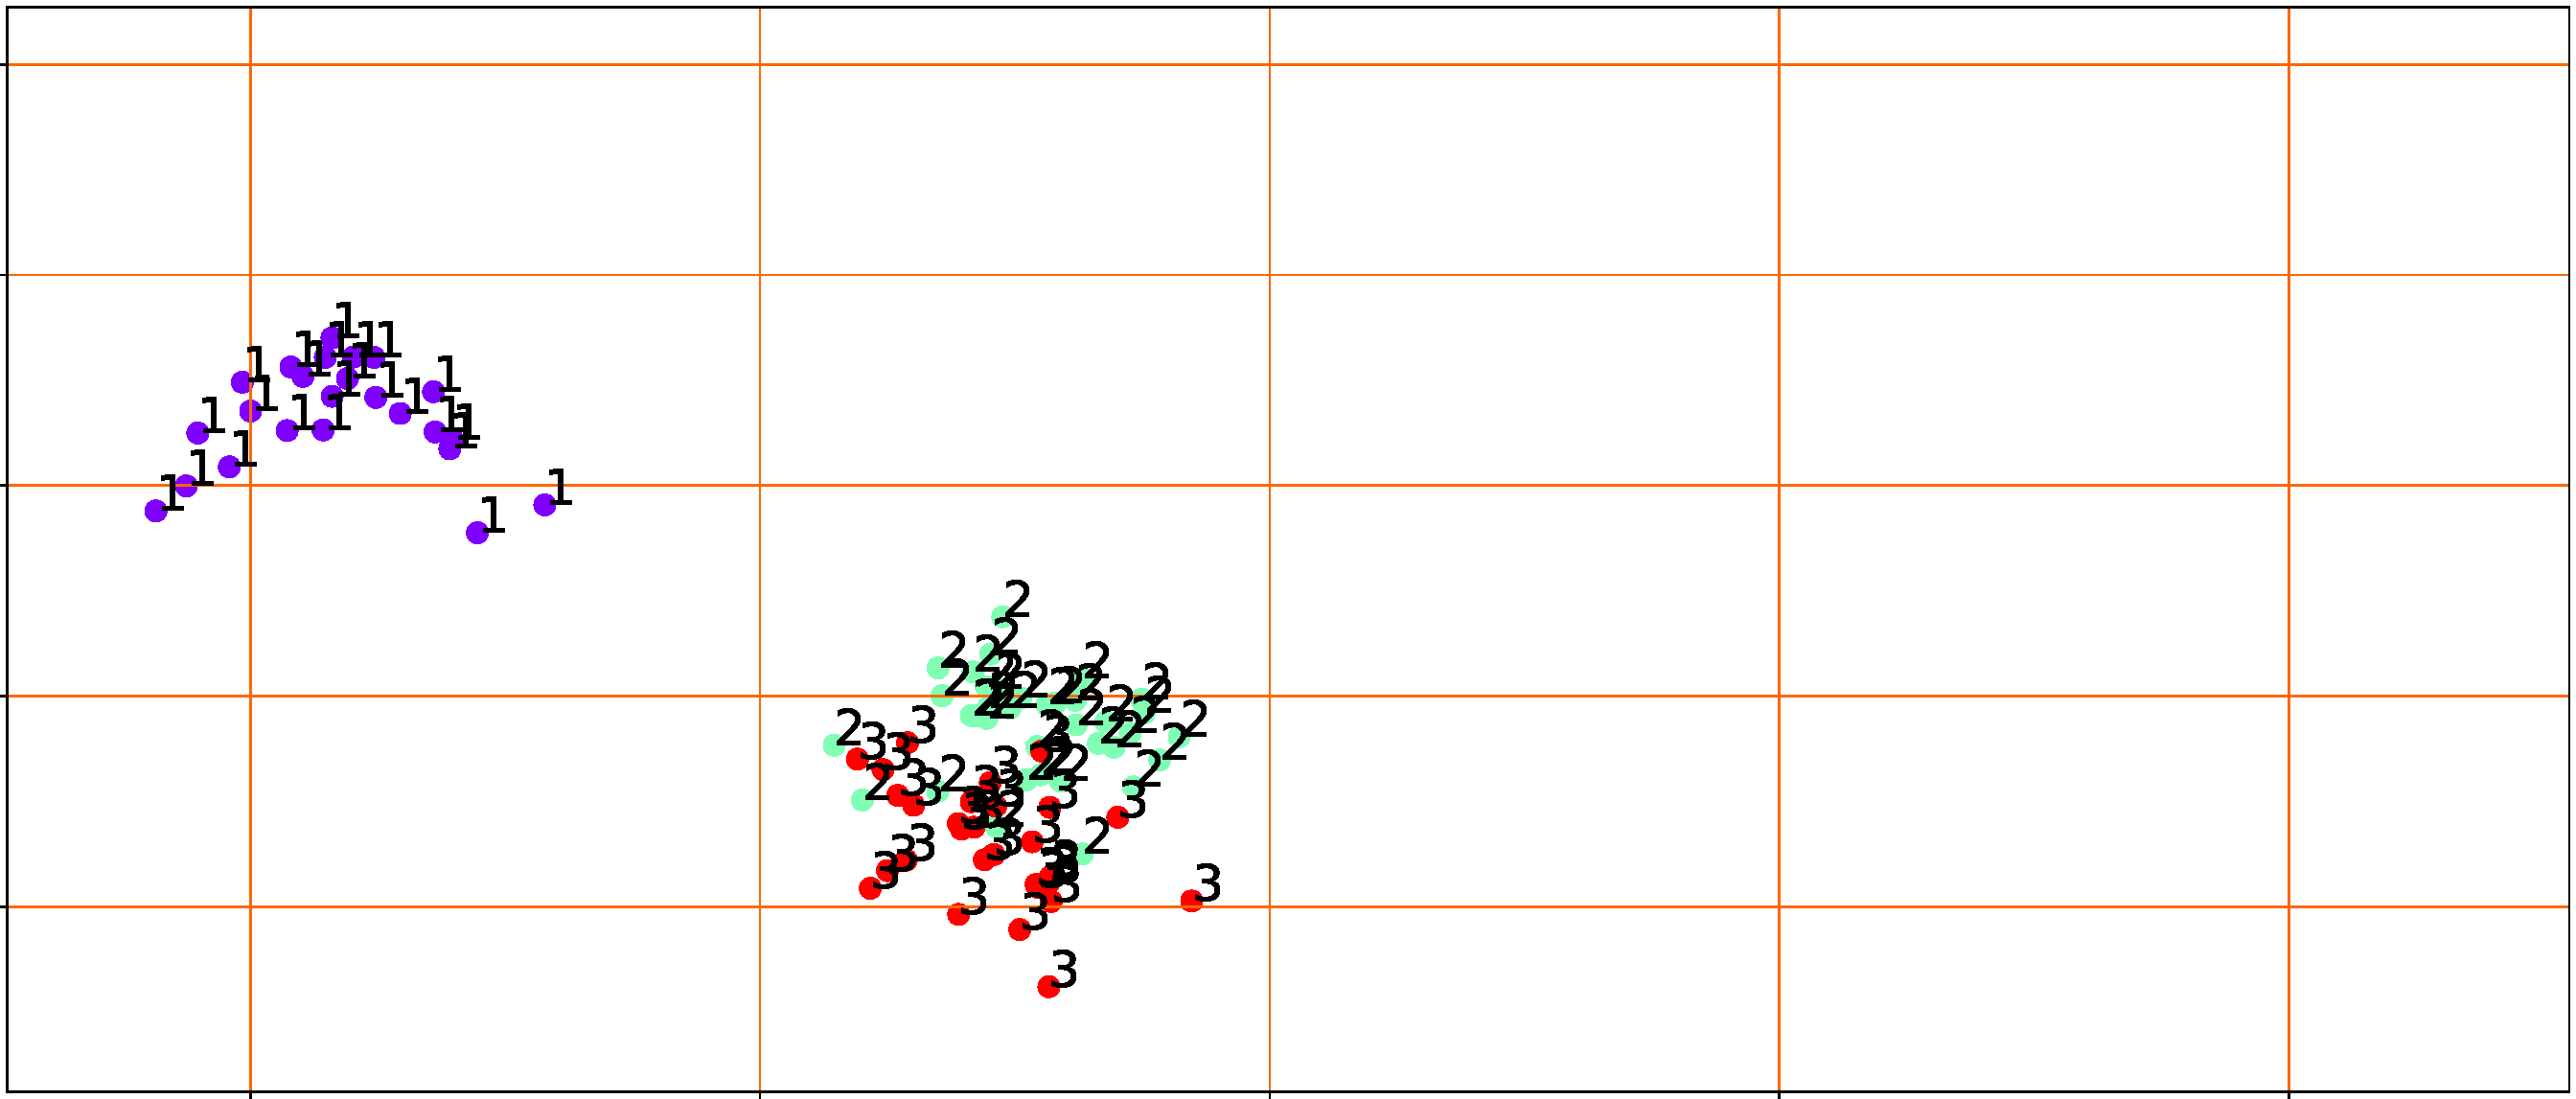
\includegraphics[width=\textwidth]{labelled-data.pdf}
	\end{figure}
\end{frame}

\begin{frame}{Random Forests}{A yoghurt example}
	\begin{figure}
		\centering
		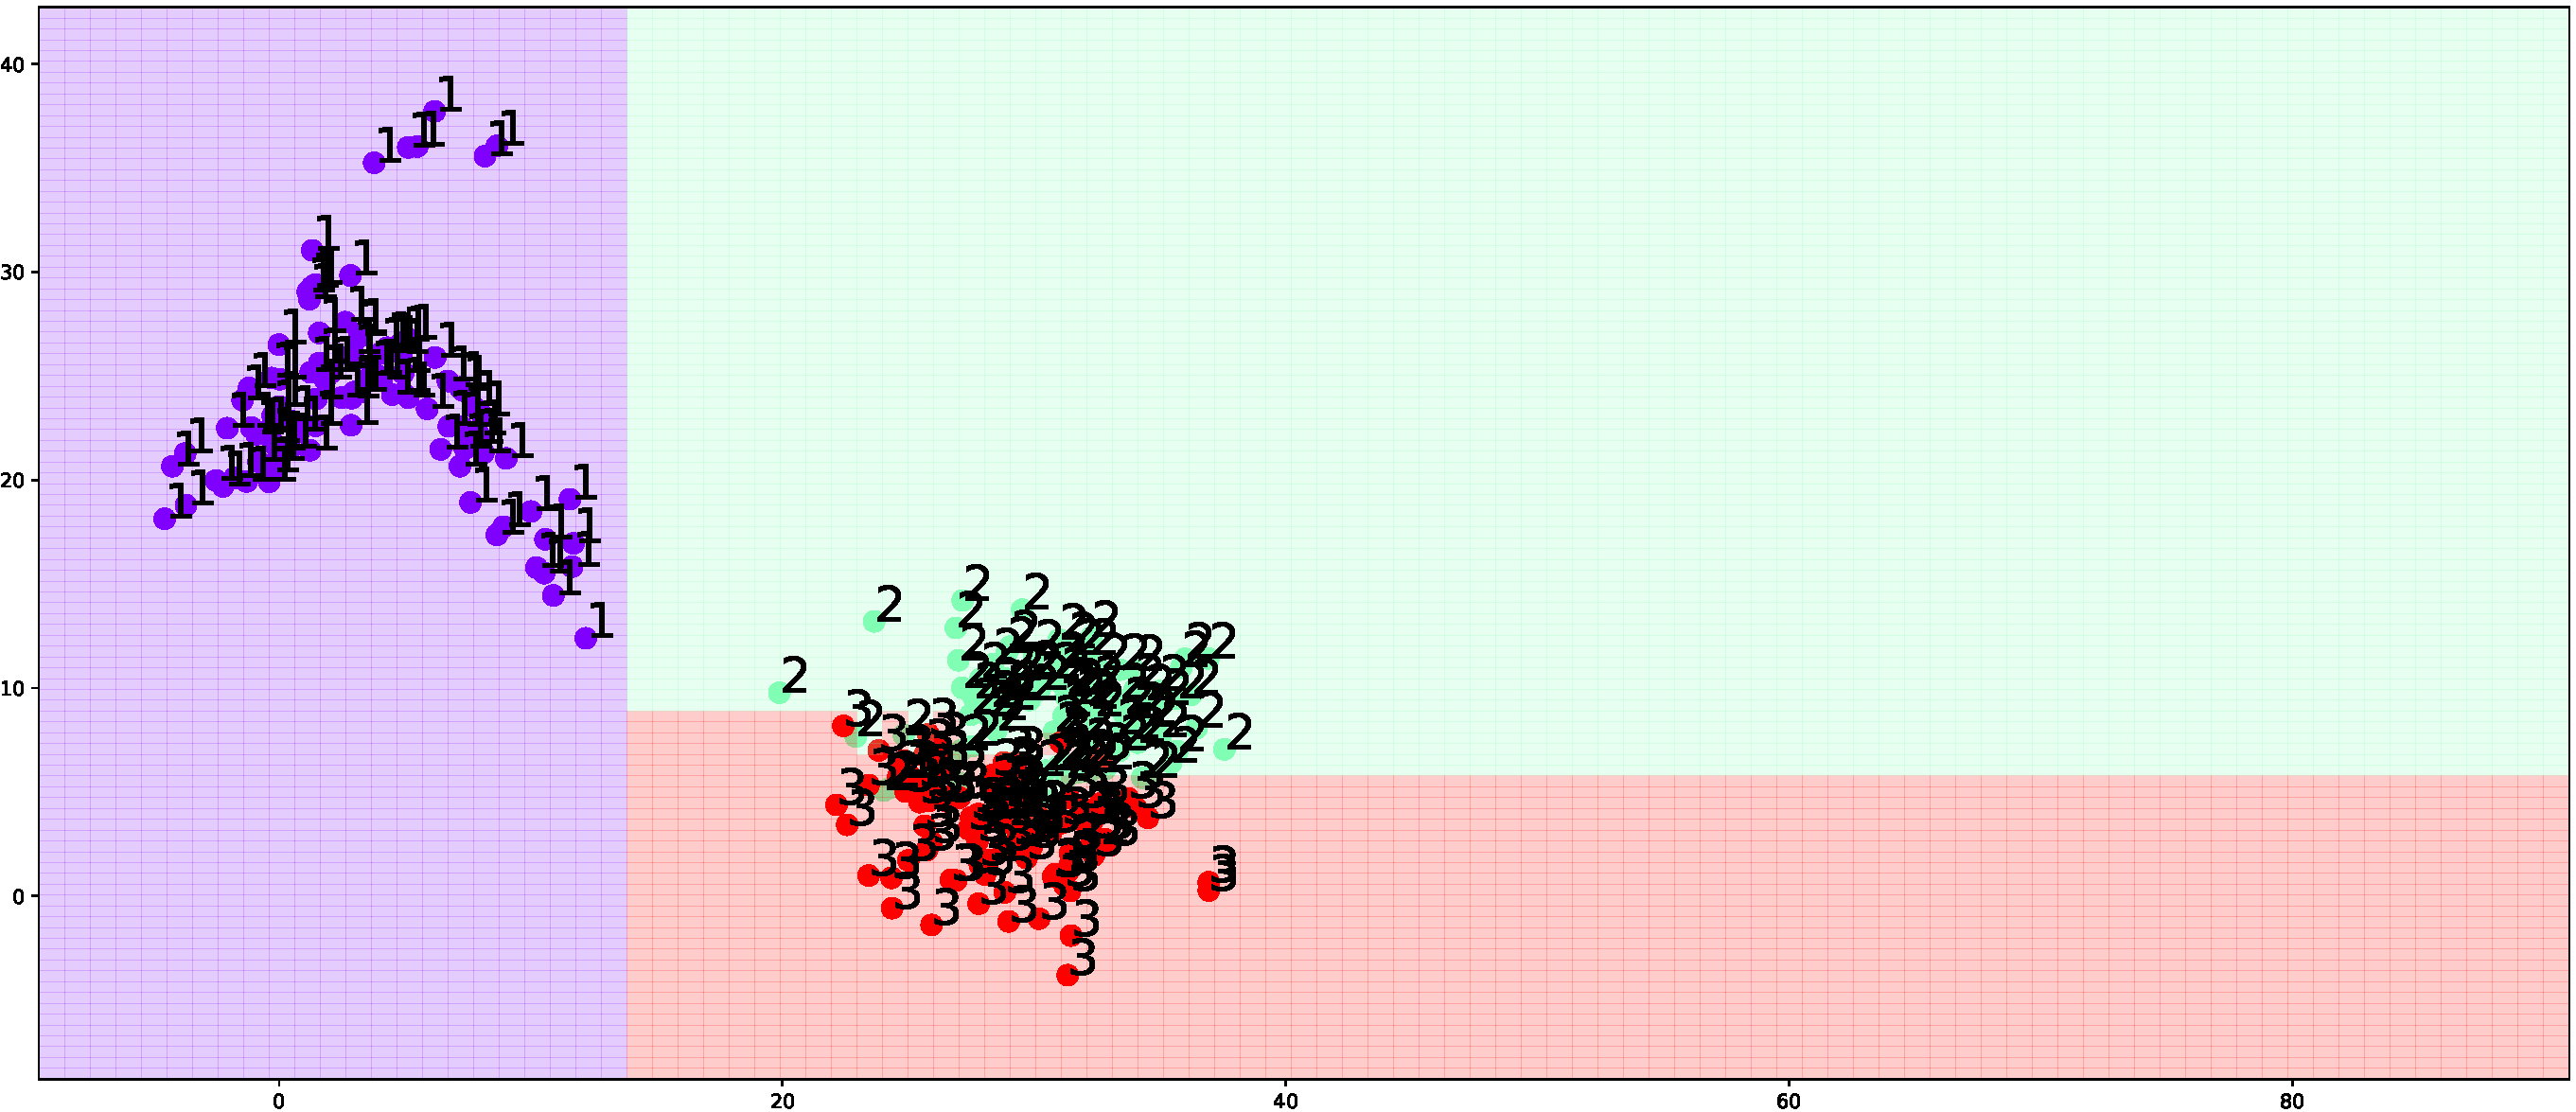
\includegraphics[width=\textwidth]{decision_boundaries}
		\caption{Single Decision Tree}
	\end{figure}
\end{frame}

\begin{frame}{Random Forests}{A yoghurt example}
	\begin{figure}
		\centering
		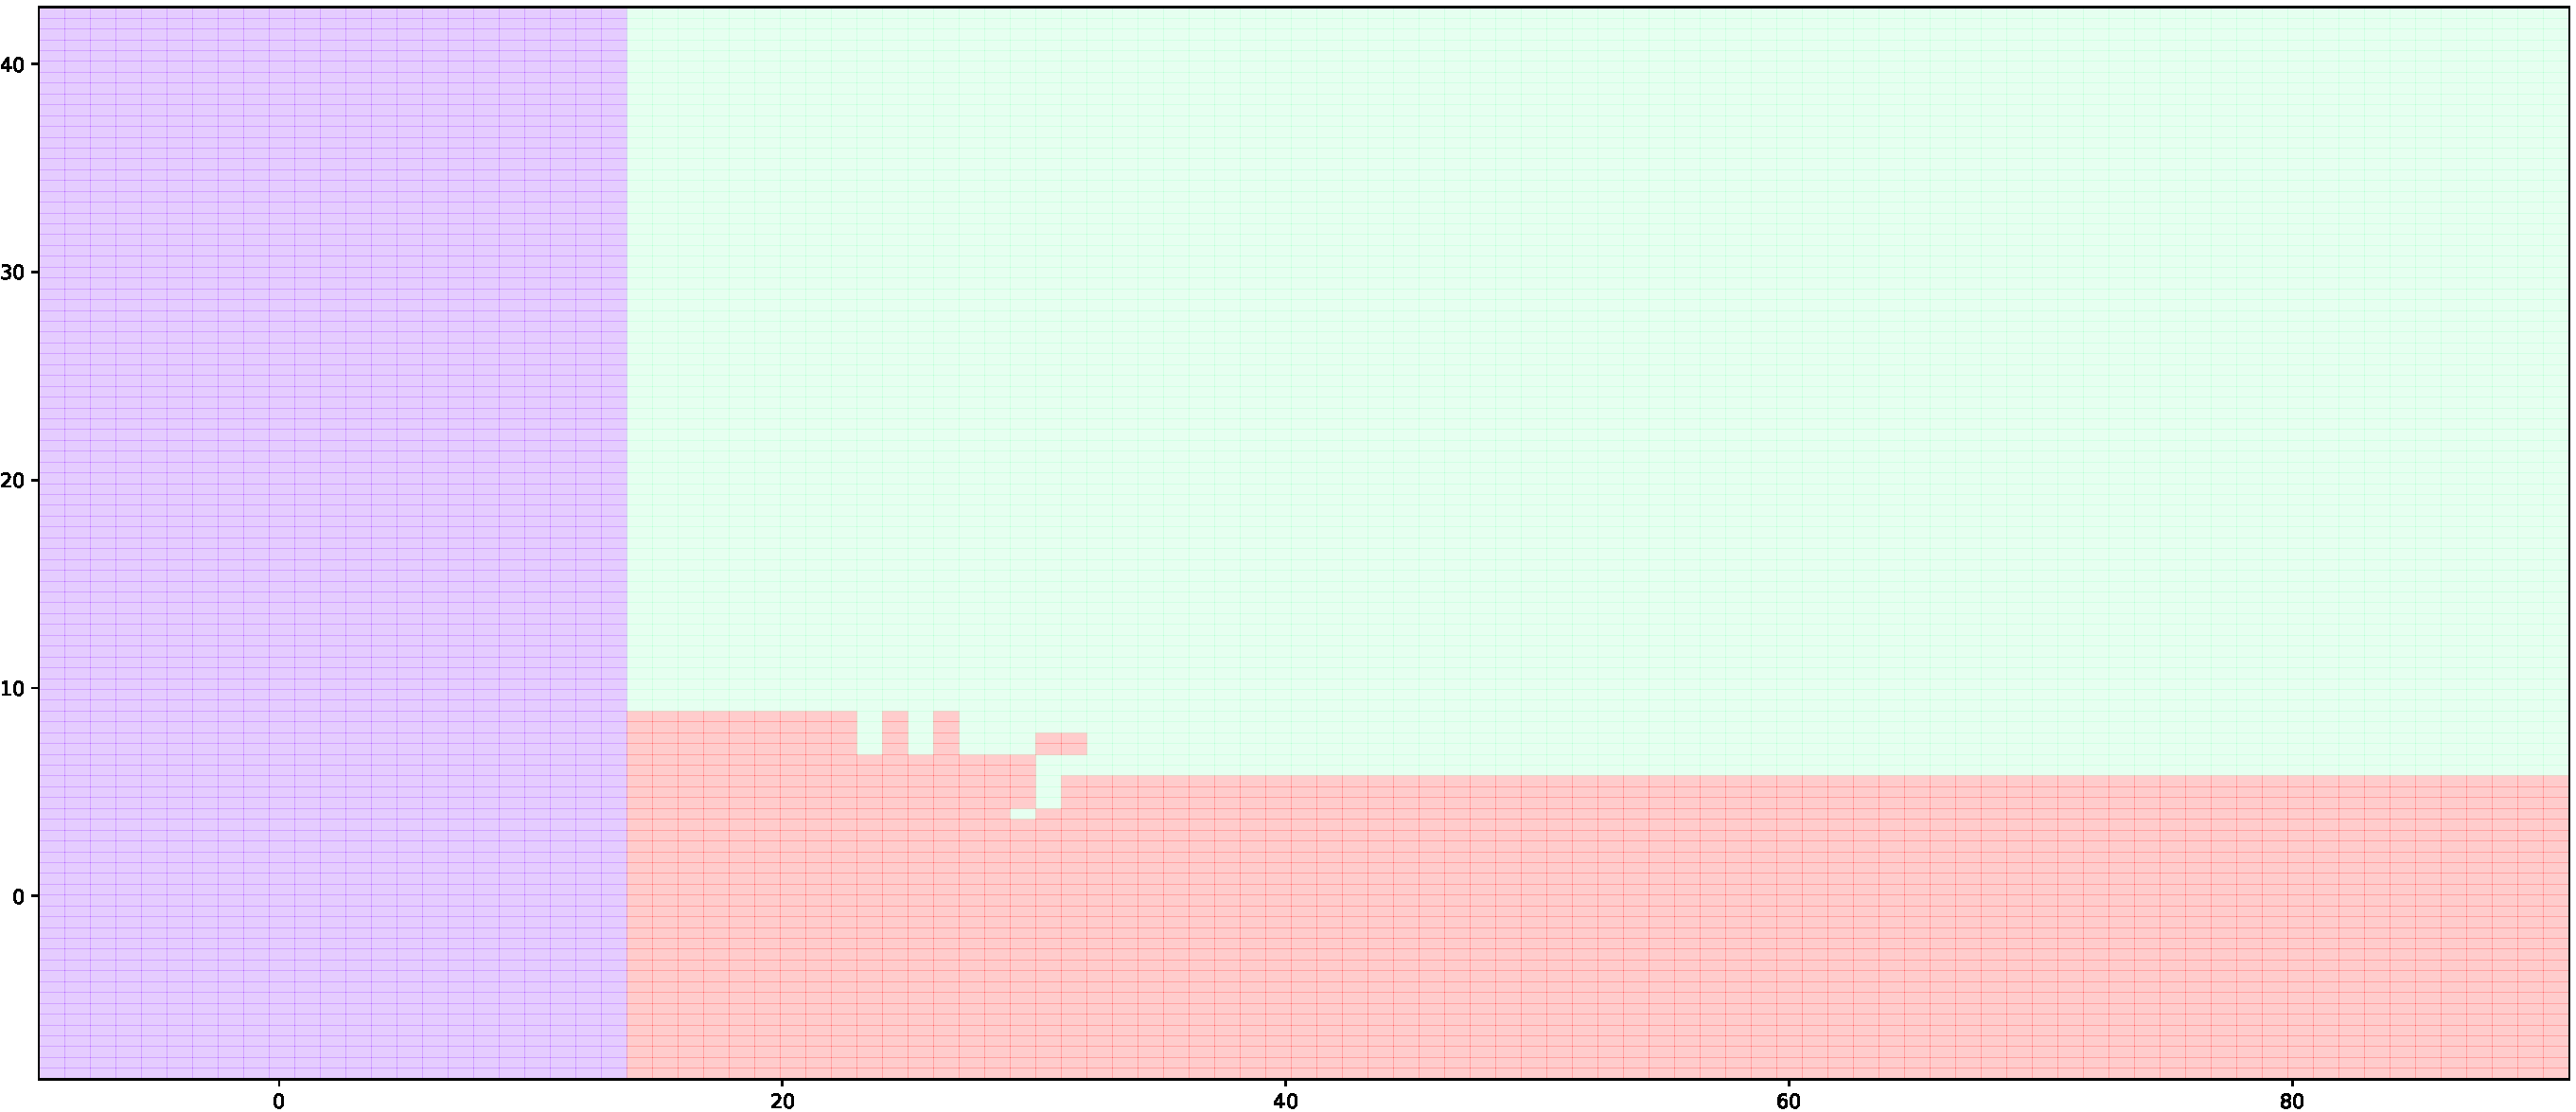
\includegraphics[width=\textwidth]{decision_boundaries_nopoints}
		\caption{Single Decision Tree}
	\end{figure}
\end{frame}

\begin{frame}{Random Forests}{A yoghurt example}
	\begin{figure}
		\centering
		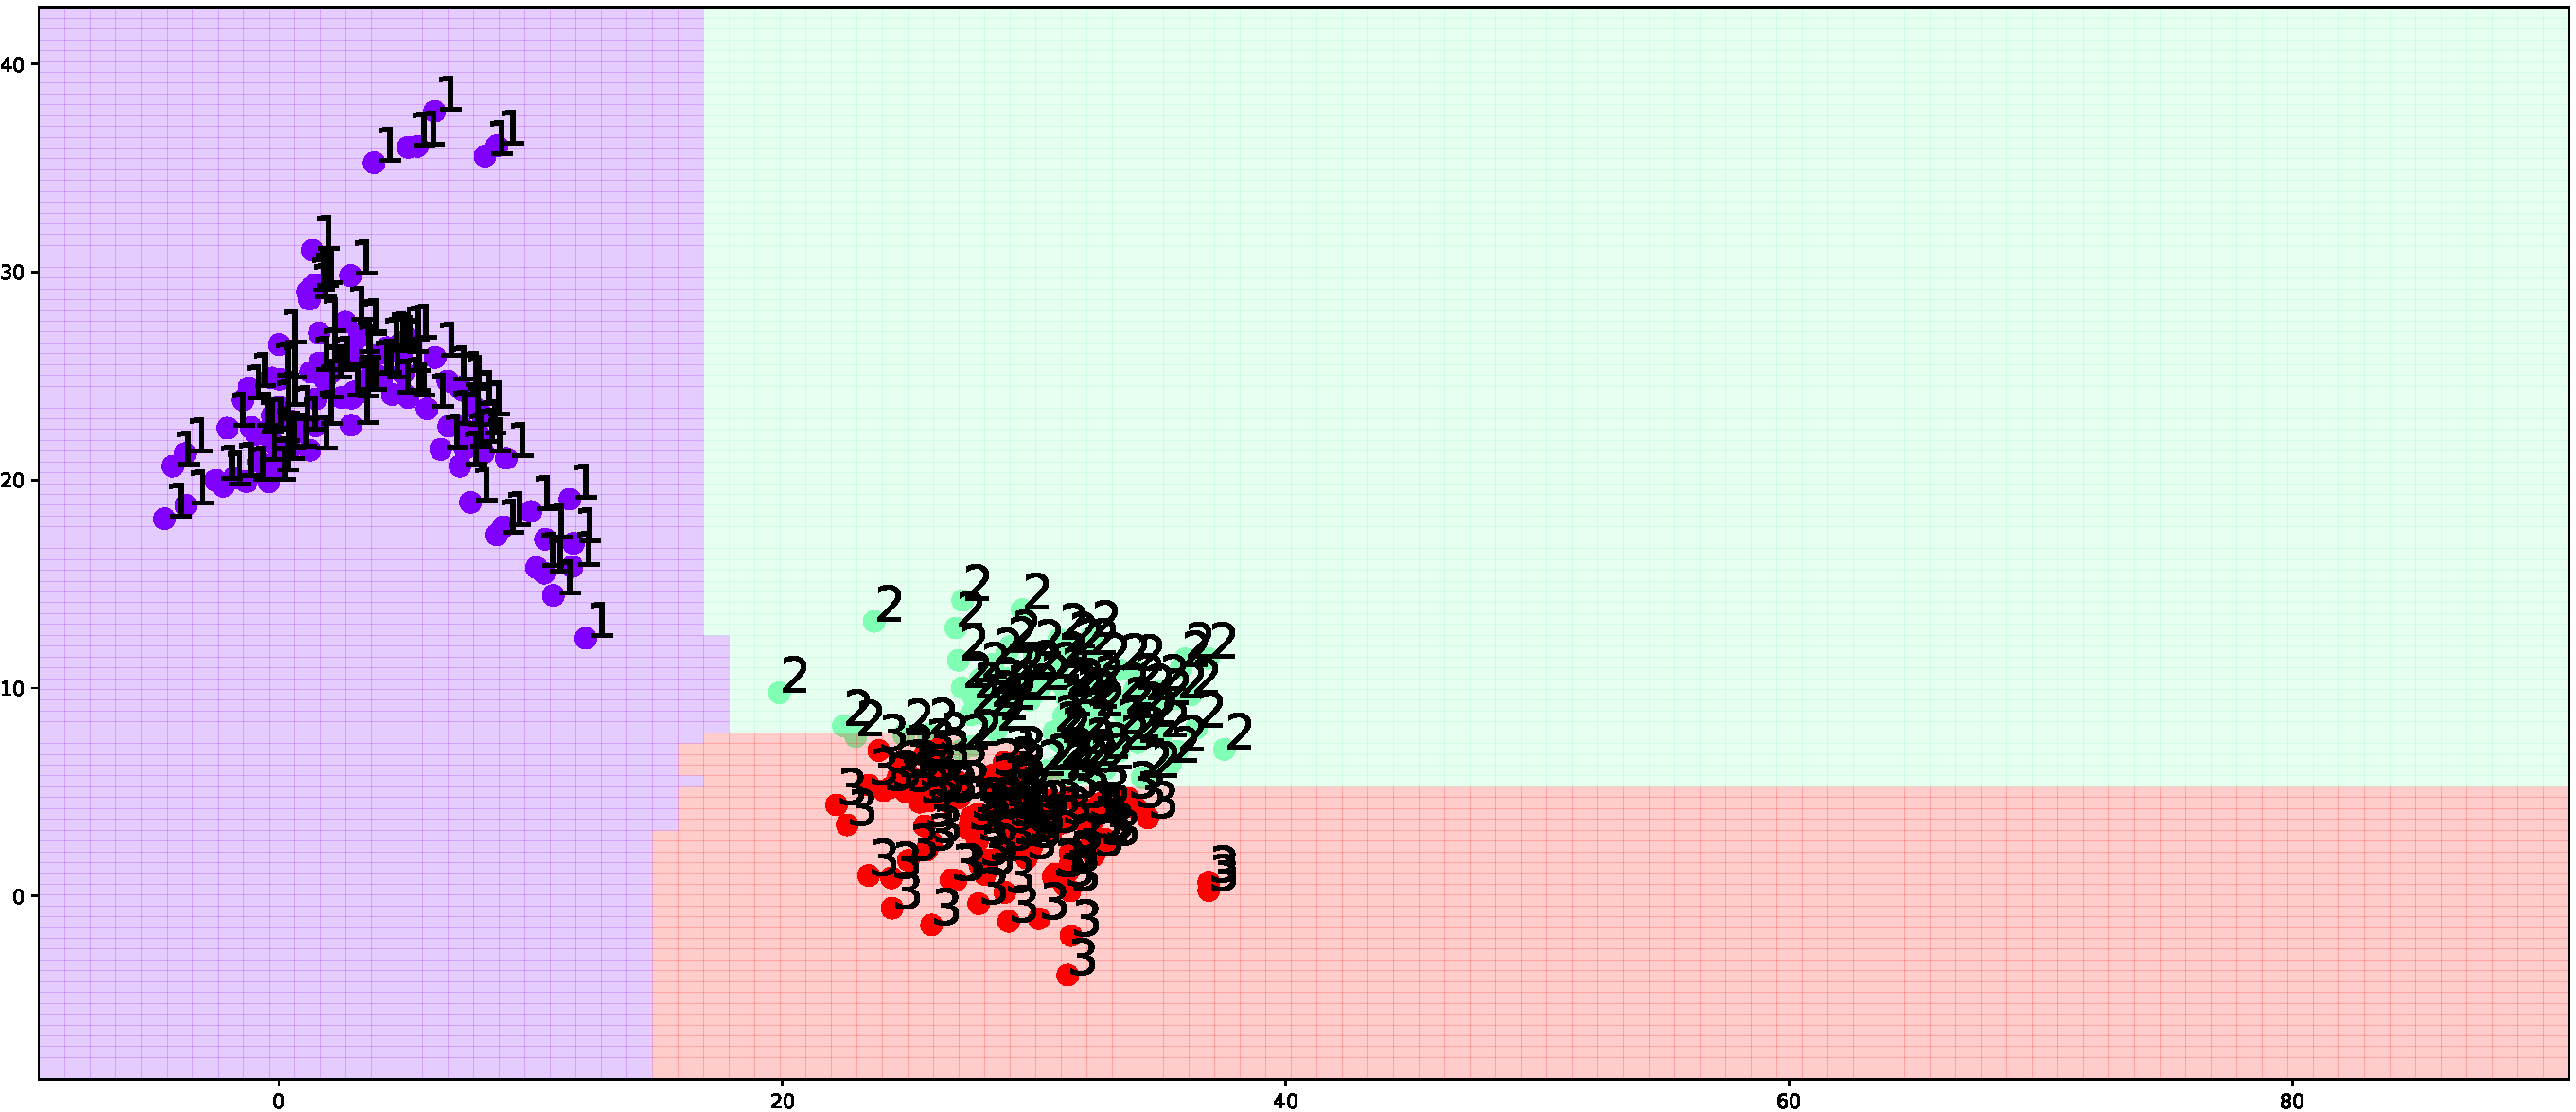
\includegraphics[width=\textwidth]{rf}
		\caption{Random Forest}
	\end{figure}
\end{frame}

\begin{frame}{Random Forests}{A yoghurt example}
	\begin{figure}
		\centering
		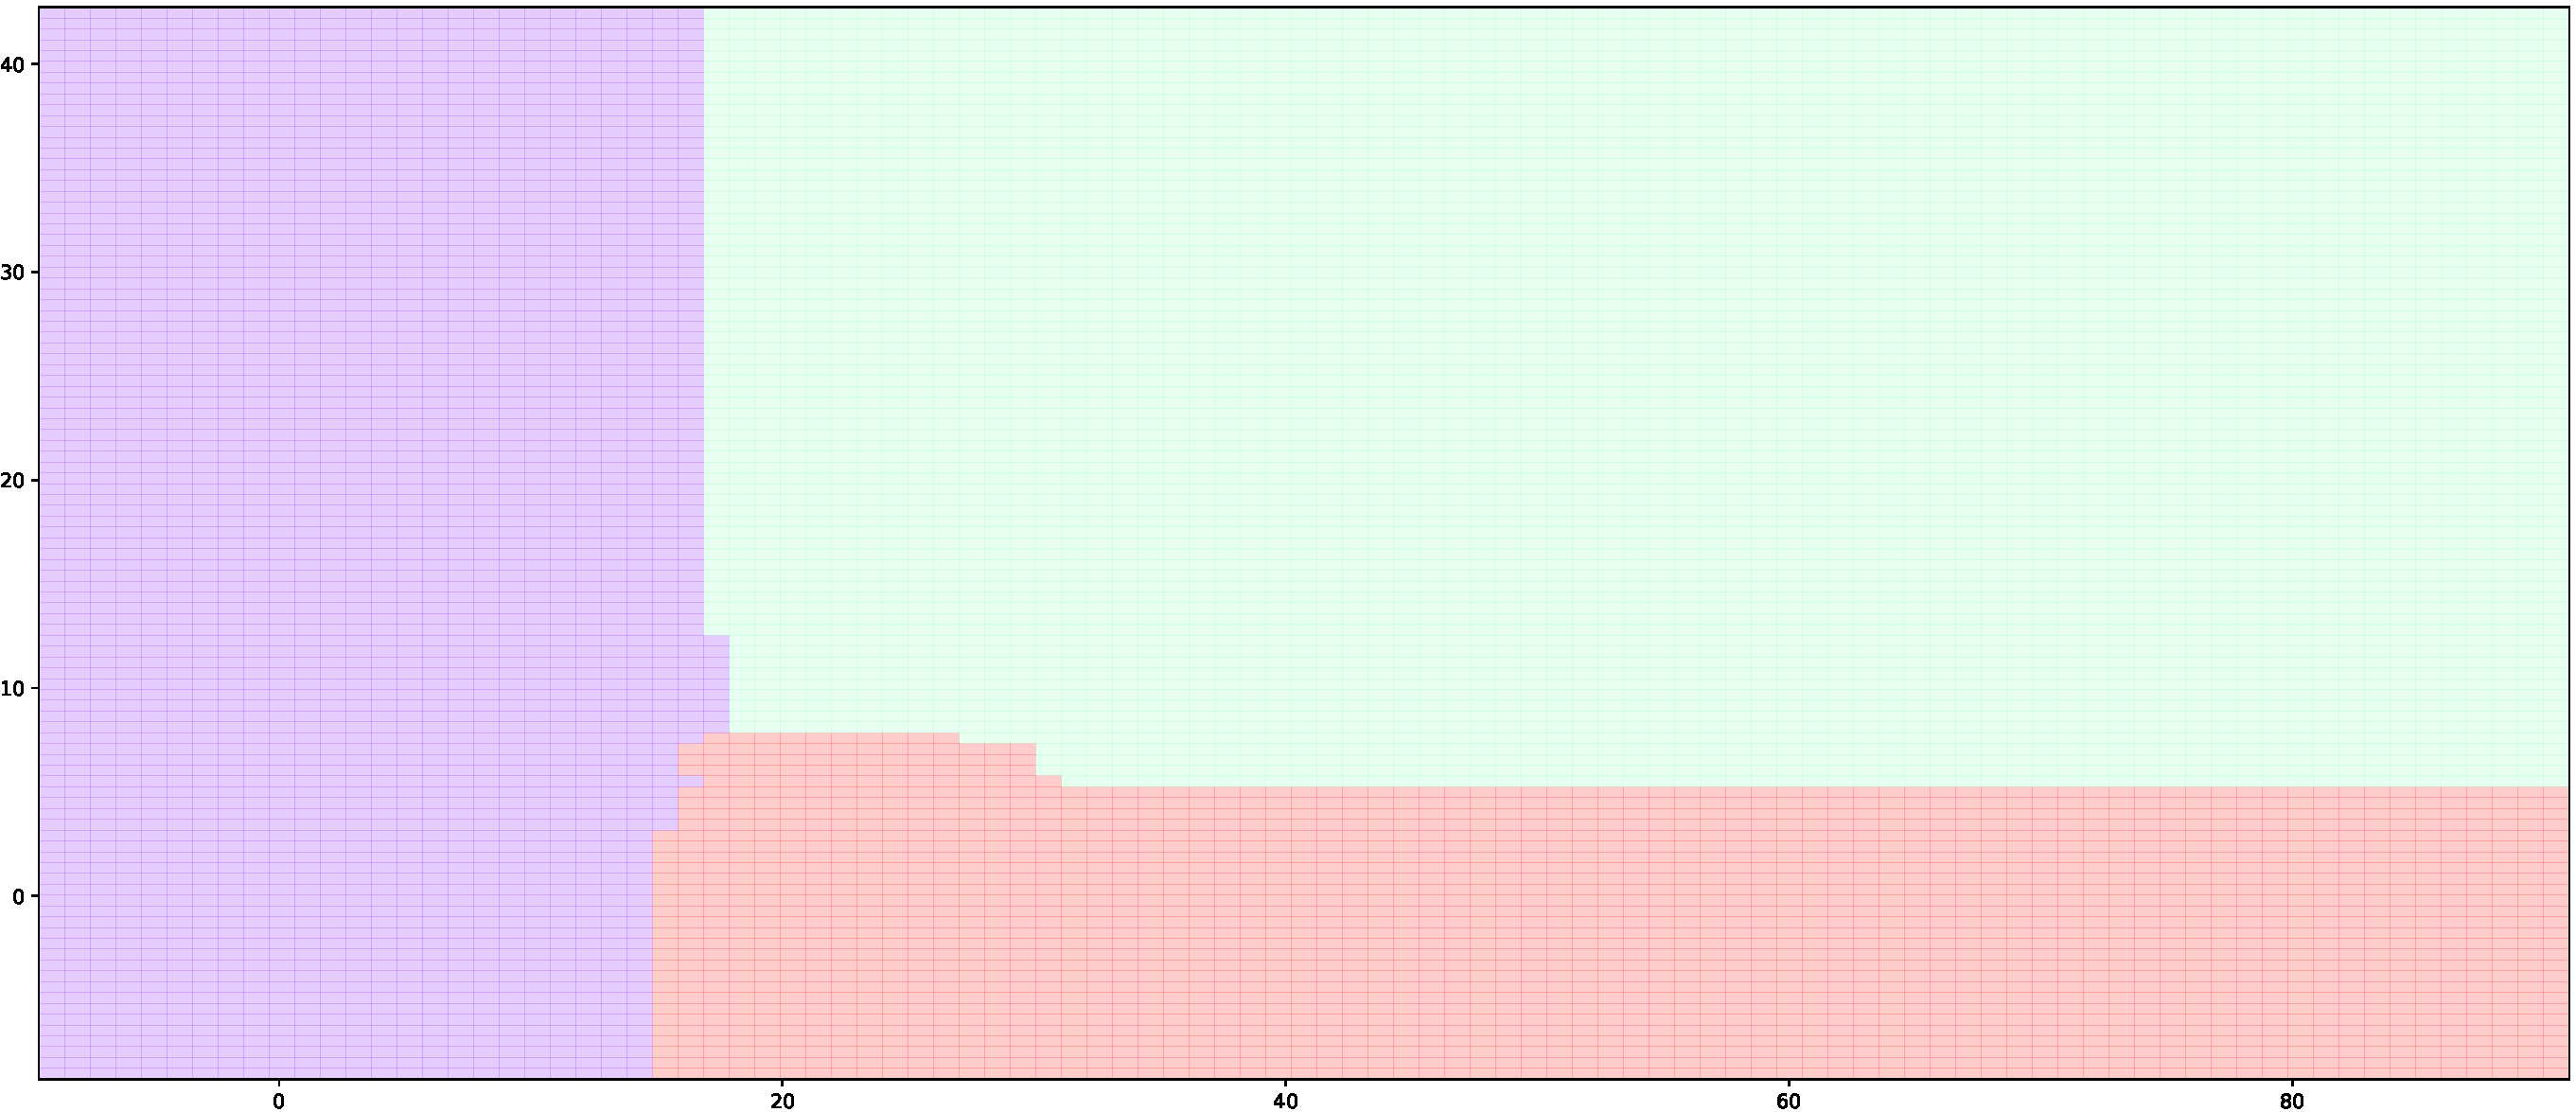
\includegraphics[width=\textwidth]{rf_nopoints}
		\caption{Random Forest}
	\end{figure}
\end{frame}

\begin{frame}{\acrlongpl{DF}}{An non-yoghurt example}
	\textbf{Question}: How to define subspaces of unlabelled data?
	\begin{figure}
		\centering
		
\includegraphics[width=\textwidth]{labelled-data-migros-new}
	\end{figure}
\end{frame}

\begin{frame}{\acrlongpl{DF}}{An non-yoghurt example}
			\begin{figure}
				\centering
				\foreach \i in {1,...,5}{
					\includegraphics<\i>[width=.5\textwidth]{df-step\i}
					\includegraphics<\i>[width=.48\textwidth]{df-step\i-tree-steps}
				}
			\end{figure}
\end{frame}

\begin{frame}{\acrlongpl{DF}}{An non-yoghurt example}
	\begin{itemize}
		\item Finding best split by maximizing \textbf{Gaussianity} at each side
		\item \textbf{Bagging} (\textbf{B}ootstrap \textbf{Agg}regat\textbf{ing}) of multiple weak learners
	\end{itemize}
	$\Rightarrow$ Requires tuning \textbf{hyperparameters} to avoid under- and overfitting:
	\begin{itemize}	
		\item Number of trees
		\item Tree depth
		\item Number of dimensions to consider for splitting
	\end{itemize}
\end{frame}

\subsection{Datasets}

% Synthetic dataset
\begin{frame}{Datasets}{Synthetic Datasets}
\vspace{-20pt}
\begin{figure}

\centering
\foreach \dataset in {1,2,3}{
\includegraphics[width=.32\textwidth]{D\dataset_data.pdf}
}
\caption{Synthetic datasets}

\end{figure}
Just used to illustrate \acrlongpl{DF}.

\end{frame}

% MNIST dataset
\begin{frame}{Datasets}{\gls{MNIST} \cite{mnist}}

% MNIST images
\begin{figure}[H]
	\centering
	% loop rows
	\foreach \j in {0,...,2}
	{
		% loop classes
		\foreach \i in {0,...,9}
		{
			\begin{subfigure}{.08\textwidth}
				\centering
				\includegraphics[width=\textwidth]{MNIST_cl_\i_\j}
			\end{subfigure}
		}
		\\
	}
\end{figure}
\vfill
60'000 training images, 10'000 test images, classes balanced
\vfill
\end{frame}

% Zurich dataset
\begin{frame}{Datasets}{Zurich Dataset \cite{Volpi2015SemanticSO}}

\begin{figure}[H]
	\centering
	\begin{subfigure}{0.49\textwidth}
		\caption{RGB Image}
		\includegraphics[width=\textwidth]{Im_16}
	\end{subfigure}
	\begin{subfigure}{0.49\textwidth}
		\caption{\acrlong{GT}}
		\includegraphics[width=\textwidth]{GT_16}
	\end{subfigure}
	\\[.2cm]
	\legendH
\end{figure}
\end{frame}

\newcommand{\mnistleaveoneout}[1]{  % argument: width 
	\begin{figure}[H]
		\centering
		% loop rows
		% loop classes
		% class 0
		\begin{subfigure}{#1\textwidth}
			\centering
			\includegraphics[width=\textwidth]{MNIST_cl_0_0_not}
		\end{subfigure}
		\foreach \i in {1,...,9}
		{
			\begin{subfigure}{#1\textwidth}
				\centering
				\includegraphics[width=\textwidth]{MNIST_cl_\i_0}
			\end{subfigure}
		}\\
		% class 1
		\begin{subfigure}{#1\textwidth}
			\centering
			\includegraphics[width=\textwidth]{MNIST_cl_0_0}
		\end{subfigure}
		\begin{subfigure}{#1\textwidth}
			\centering
			\includegraphics[width=\textwidth]{MNIST_cl_1_0_not}
		\end{subfigure}
		\foreach \i in {2,...,9}
		{
			\begin{subfigure}{#1\textwidth}
				\centering
				\includegraphics[width=\textwidth]{MNIST_cl_\i_0}
			\end{subfigure}
		}\\
		% class 2
		\foreach \i in {0,1}
		{
			\begin{subfigure}{#1\textwidth}
				\centering
				\includegraphics[width=\textwidth]{MNIST_cl_\i_0}
			\end{subfigure}
		}
		\begin{subfigure}{#1\textwidth}
			\centering
			\includegraphics[width=\textwidth]{MNIST_cl_2_0_not}
		\end{subfigure}
		\foreach \i in {3,...,9}
		{
			\begin{subfigure}{#1\textwidth}
				\centering
				\includegraphics[width=\textwidth]{MNIST_cl_\i_0}
			\end{subfigure}
		}\\
		$\boldsymbol{\vdots}$\\
		% class 9
		\foreach \i in {0,...,8}
		{
			\begin{subfigure}{#1\textwidth}
				\centering
				\includegraphics[width=\textwidth]{MNIST_cl_\i_0}
			\end{subfigure}
		}
		\begin{subfigure}{#1\textwidth}
			\centering
			\includegraphics[width=\textwidth]{MNIST_cl_9_0_not}
		\end{subfigure}
	\end{figure}
}


\subsection{Experimental Setup}
\begin{frame}{Experimental Setup}{CNN}
	\glspl{CNN}
	\begin{itemize}
		\item Standard network architectures
		\item Leaving one class out during training
	\end{itemize}
	\mnistleaveoneout{.06}
\end{frame}
\begin{frame}{Experimental Setup}{CNN}
\glspl{CNN}
	\begin{itemize}
		\item Standard network architectures
		\item Leaving one class out during training
	\end{itemize}	
		\begin{figure}[H]
			\begin{subfigure}{.4\textwidth}
				\centering
				\includegraphics<1->[width=\textwidth]{GT_14.jpg}
			\end{subfigure}
			$\Rightarrow$
			\begin{subfigure}{.4\textwidth}
				\centering\includegraphics<1>[width=\textwidth]{GT_14_wo_cl_1}\includegraphics<2>[width=\textwidth]{GT_14_wo_cl_2}\includegraphics<3>[width=\textwidth]{GT_14_wo_cl_3}
			\end{subfigure}
		\end{figure}
\end{frame}

\begin{frame}{Experimental Setup}{CNN}
	Novelty Detection methods \gls{GMM}, \gls{OC-SVM}, \gls{DF}
	\begin{itemize}
		\item Model activations of the \textit{seen classes}
		\item Predicting confidence for entire test set, including the \textit{unseen class}
	\end{itemize}
\end{frame}

\begin{frame}{Experimental Setup}{Dimensionality Reduction}
	\begin{itemize}
		\item Standard \gls{CNN} for \gls{MNIST} yields 128 activations\\
		\begin{itemize}
			\item Redundancy, collinearity
			\item High-dimensional data difficult to handle
		\end{itemize}
		\item \gls{PCA}: preserve data variance
		\item Visualization: \gls{t-SNE}
	\end{itemize}
	
	\begin{figure}[H]
		\centering
		\includegraphics[width=.8\textwidth]{t-SNE-schema}
	\end{figure}
\end{frame}



\subsection{Evaluation}
\begin{frame}{Evaluation}
	\begin{itemize}
		\item \textbf{U-Net \gls{CNN}} models with left-out class: \gls{OA}, \gls{AA}
		\item \textbf{Novelty Detection}:
		\begin{itemize}
			\item \gls{AUROC}
			\item Visual quality of results
		\end{itemize}
	\end{itemize}
\end{frame}


\begin{frame}
\begin{figure}
	\centering
	\includegraphics[height=.95\textheight]{../Report/Schema/schema_df}
\end{figure}
\end{frame}

\section{Results}

\begin{frame}{Results}
\centering
\end{frame}


\subsection{Dummy Dataset}
\begin{frame}{Dummy Dataset: One Tree}
% Splitting steps
	\vspace{-10pt}
	\begin{figure}[H]
		\centering
			\begin{subfigure}{.5\textwidth}
				\caption{\only<1>{Depth = 0}\only<2>{Depth = 1}\only<3>{Depth = 2}\only<4>{Depth = 3}\only<5>{Depth = 4}\only<6>{Gaussian \gls{PDF}}}
				\foreach \depth [count = \xi] in {0,...,4}
				{
				\includegraphics<\xi>[width=\textwidth]{D2_data_covs_depth_\depth}
				}
				\includegraphics<6>[width=\textwidth]{D2_one_tree}
			\end{subfigure}
	\end{figure}
\end{frame}
\begin{frame}{Dummy Datasets: Several Trees}
\begin{figure}[H]
	\foreach \name/\dataset/\captionname/\do in {
		one_tree/1/Density Tree/,
		one_tree/2/Density Tree/,
		one_tree/3/Density Tree/\pause,
		DF_forest/1/\acrlong{DF}/,
		DF_forest/2/\acrlong{DF}/,
		DF_forest/3/\acrlong{DF}/}
	{
		\begin{subfigure}{0.3\textwidth}
			\centering
			\includegraphics[width=\textwidth]{D\dataset_\name}
		\end{subfigure}\do
	}
\end{figure}
\end{frame}

\subsection{MNIST Dataset}
\begin{frame}{\gls{MNIST} Dataset}{\glspl{CNN}}
	\glspl{CNN} trained leaving out one class
	\pause
	% MNIST images
	\mnistleaveoneout{.06}
	\pause
	Accuracy:
	\begin{table}[H]
		\centering
		\begin{tabular}{cc}
			\toprule
			Training set & Test set \\\midrule
			99.34 & 99.03  \\\bottomrule
		\end{tabular}
	
		\label{table:mnist-nd-accuracy-mean}
	\end{table}
	High accuracy, but...
\end{frame}


\begin{frame}{\gls{MNIST}}{\gls{t-SNE}}
	% Class 7 before and after PCA
	\begin{figure}[H]
		\centering
		\begin{subfigure}{.49\textwidth}
			\centering
			\includegraphics[width=\textwidth]{MNIST_t-SNE_wo_cl_7_before}
			\caption{\acrshort{t-SNE} before \acrshort{PCA}}
		\end{subfigure}
		\begin{subfigure}{.5\textwidth}
			\centering
			\includegraphics[width=\textwidth]{MNIST_t-SNE_wo_cl_7_after}
			\caption{\acrshort{t-SNE} after \acrshort{PCA}}
		\end{subfigure}
		\\[.2cm]
		\legendBulletMNIST (class 7)
		\label{fig:tsne-mnist}
	\end{figure}
\end{frame}

\begin{frame}{\gls{MNIST}}{Novelty Detection}
\begin{table}[H]
	\centering
	\begin{tabular}{@{}llll|lll@{}}
		\toprule
		\gls{MSR}  & Margin & Entropy & \gls{MC-Dropout} & \gls{GMM} & \gls{OC-SVM}  & \gls{DF} \\ \midrule
		\textbf{0.97} & \textbf{0.97} & \textbf{0.97} & 0.96 & 0.67 & 0.75 & 0.75 \\\bottomrule
	\end{tabular}
	\caption{Mean \gls{AUROC} for each left-out class in the \gls{MNIST} dataset}
	\label{table:mnist-auroc-nd-mean}
\end{table}
\pause
\centering 
:/ \\

We'll come back to this...
\end{frame}
	

\subsection{Zurich Dataset}
	\begin{frame}{Zurich Dataset}{\glspl{CNN}}
	\begin{figure}[H]
		\centering
		\begin{subfigure}{0.49\textwidth}
			\caption{\acrlong{GT}}
			\pdfpxdimen=\dimexpr 1 in/255\relax
			\includegraphics<1->[clip, trim=0 523px 310px 0, width=\textwidth]{GT_16}
		\end{subfigure}
		\begin{subfigure}{0.49\textwidth}
			\caption{\only<1>{Prediction (wo. Roads)}\only<2>{Prediction (wo. Buildings)}\only<3>{Prediction (wo. Trees)}}
			\foreach \i in {1,...,3}{\pdfpxdimen=\dimexpr 1 in/255\relax
				\includegraphics<\i>[clip, trim=0 523px 310px 0, width=\textwidth]{Im_16_wo_cl_\i}}
		\end{subfigure}
		\\[.2cm]
		\legendH
	\end{figure}
\end{frame}

\begin{frame}{Novelty Detection}{Are the activations separable?}
% t-SNE, separable before and after t-SNE
\begin{figure}[H]
	\centering
	\begin{subfigure}{.48\textwidth}
		\centering
		\caption{\gls{t-SNE} before \gls{PCA}}
		\includegraphics[width=\textwidth]{t-SNE_wo_cl2_before_PCA}
	\end{subfigure}
	\begin{subfigure}{.48\textwidth}
		\centering
		\caption{\gls{t-SNE} after \gls{PCA}}
		\includegraphics[width=\textwidth]{t-SNE_wo_cl2_after_PCA}
	\end{subfigure}
	\legendBullet
	\label{fig:tsne-zurich}
\end{figure}
\end{frame}


\begin{frame}{Novelty Detection}{Unseen Class \textbf{Roads}}
	\begin{figure}[H]
		\centering
		\begin{subfigure}{0.49\textwidth}
			\caption{\acrlong{GT}}
			\pdfpxdimen=\dimexpr 1 in/255\relax
			\includegraphics<1->[clip, trim=0 523px 310px 0, width=\textwidth]{GT_16}
		\end{subfigure}
		\begin{subfigure}{0.49\textwidth}
			\caption{\only<1>{\gls{MSR}}\only<2>{\gls{OC-SVM}}\only<3>{\gls{DF}}}
			\foreach \i/\method in {1/net_msr_im_1,2/svm_im_1_eq,3/df_im_1_eq}{\pdfpxdimen=\dimexpr 1 in/255\relax
				\includegraphics<\i>[clip, trim=0 523px 310px 0, width=\textwidth]{ZH_wo_cl_1_\method}}
		\end{subfigure}
		\\[.1cm]
		\legendGTandCert
	\end{figure}
\end{frame}

\newcommand{\ndResults}[5]{  % class, class name, image, gt, trim
	\begin{frame}{Novelty Detection}{Unseen Class \textbf{#2}}
		\begin{figure}[H]
			\centering
			\begin{subfigure}{0.32\textwidth}
				\centering
				\pdfpxdimen=\dimexpr 1 in/255\relax
				\includegraphics[clip, trim=#5, width=\textwidth]{ZH_wo_cl_#1_net_msr_im_#3}
				\caption{MSR}
			\end{subfigure}
			\begin{subfigure}{0.32\textwidth}
				\centering
				\pdfpxdimen=\dimexpr 1 in/255\relax
				\includegraphics[clip, trim=#5, width=\textwidth]{ZH_wo_cl_#1_svm_im_#3_eq}
				\caption{\gls{OC-SVM}}
			\end{subfigure}
			\begin{subfigure}{0.32\textwidth}
				\centering
				\pdfpxdimen=\dimexpr 1 in/255\relax
				\includegraphics[clip, trim=#5, width=\textwidth]{ZH_wo_cl_#1_df_im_#3_eq}
				\caption{\gls{DF}}
			\end{subfigure}
			\begin{subfigure}{0.5\textwidth}
				\centering
				\pdfpxdimen=\dimexpr 1 in/255\relax
				\includegraphics[clip, trim=#5, width=\textwidth]{GT_#4}
			\end{subfigure}
			\begin{subfigure}{0.4\textwidth}
				\centering
				\includegraphics[width=\textwidth]{ROC_pred_wo_cl_#1}
			\end{subfigure}
		\end{figure}
	\end{frame}
}

\ndResults{1}{Roads}{1}{16}{0 523px 310px 0}
\ndResults{6}{Water}{0}{15}{0 0 0 600px}

% TODO add other class

\newcommand{\tick}{${\color[rgb]{0, .5, 0}\mathbf{\checkmark}}$}

\begin{frame}{Novelty Detection}{Best Uncertainty Measures}
	\begin{table}[H]
		\centering
		\footnotesize
		\begin{tabular}{@{}l|llll|lll@{}}
			\toprule
			Left-Out Class & MSR  & Margin     & Entropy & \gls{MC-Dropout} & \gls{GMM}     & \gls{OC-SVM}  & \gls{DF}                \\ \midrule
			Roads          &   &    &     &   &  &  &  \tick \\
			Buildings    & \tick  &    &     &   &  &  &   \\
			Trees          &   &    &     &   &  &   \tick &\\ 
			Grass          &   &    &     &   &  &  &  \tick \\ 
			Bare Soil      &   & \tick   &     &   &  &  &   \\ 
			Water          &   &    &     &   &  &  \tick &   \\ 
			Railways       &   &    &     &   &  & \tick &   \\ 
			Swimming Pools &   &    &     &   &  \tick  &  &  \tick \\ \midrule
			Average       &   &    &     &   &  &  \tick &   \tick \\ \bottomrule
		\end{tabular}
	\end{table}
	\pause
	\centering
	:)
\end{frame}

\begin{frame}{Particular Objects}{Histogram Stretching}
% t-SNE, separable before and after t-SNE
\begin{figure}[H]
		\centering
		
		\begin{subfigure}{.48\textwidth}
			\centering
			\includegraphics[width=.48\textwidth]{Skew_GMM_wo_cl1}
		\end{subfigure}
		\begin{subfigure}{.48\textwidth}
			\centering
			\includegraphics[width=.48\textwidth]{Skew_GMM_wo_cl1_eq}
		\end{subfigure}\\
		\begin{subfigure}{.45\textwidth}
			\centering
			\pdfpxdimen=\dimexpr 1 in/255\relax
			\includegraphics[clip, trim=0 23px 310px 500px, width=\textwidth]{ZH_wo_cl_1_df_im_1}
			\caption{Original}
			\label{subfig:original-im}
		\end{subfigure}
		\begin{subfigure}{.45\textwidth}
			\centering
			\pdfpxdimen=\dimexpr 1 in/255\relax
			\includegraphics[clip, trim=0 23px 310px 500px, width=\textwidth]{ZH_wo_cl_1_df_im_1_eq}
			\caption{Equalized}
			\label{subfig:equalized-im}
		\end{subfigure}
		\textsc{Certainty (\acrshort{DF}, left-out class ``roads'')}\\[.2cm]
		\legendCert
	\end{figure}
\end{frame}

\newcommand{\imObject}[3]{  % args: im, obj, cl
	\begin{frame}{Zurich Dataset}{Particular Objects}
		\begin{figure}[H]
			\centering
			\begin{subfigure}{.45\textwidth}
				\centering
				\includegraphics[width=\textwidth]{im_#1_obj_#2_overlay}
				\caption{Image with \gls{ROI}}
			\end{subfigure}
			\begin{subfigure}{.45\textwidth}
				\centering
				\includegraphics[width=\textwidth]{im_#1_obj_#2_gt.jpg}
				\caption{\acrlong{GT}}
			\end{subfigure}
			\\[.2cm]
			\legendH
		\end{figure}
	\end{frame}
	\begin{frame}{Zurich Dataset}{Particular Objects}
		\begin{figure}[H]
			\centering
			\begin{subfigure}{.49\textwidth}
				\centering
				\includegraphics[width=\textwidth]{im_#1_obj_#2_msr_wo_cl_#3}
				\caption{MSR}
			\end{subfigure}
			\begin{subfigure}{.49\textwidth}
				\centering
				\includegraphics[width=\textwidth]{im_#1_obj_1_df_wo_cl_#3}
				\caption{\acrlong{DF} (non-equalized)}
			\end{subfigure}
			\\[.2cm]
			\footnotesize{\textsc{Confidence}}\\[.2cm]
			\legendCert
		\end{figure}
	\end{frame}
}
\imObject{1}{1}{4}
\imObject{4}{1}{8}

\section{Discussion}
\begin{frame}{Discussion}
Winning methods
	\begin{itemize}
		\item \gls{MNIST} dataset: softmax-based methods
		\item Zurich dataset: pre-softmax-based methods
		\begin{itemize}
			\item \gls{OC-SVM} and \acrlong{DF} work particularly well
		\end{itemize}
	\end{itemize}
\end{frame}

\begin{frame}{Varying Performance}{MNIST and Zurich dataset}
Intuitions
	% TODO add figures
	\begin{itemize}
		\item Number of pre-softmax activations
		\begin{itemize}
			\item \gls{MNIST}: 128 components, Zurich: 32 components
			\item Curse of Dimensionality
		\end{itemize}
		\item Data complexity
		% Data further away from each other?
	\end{itemize}
\end{frame}
\begin{frame}{Varying Performance}{Zurich Dataset}
	\begin{itemize}
		\item Class imbalance and class separability
		\begin{itemize}
			\item Similar classes: Roads and buildings, trees and grass
			\item Distinctive classes: Bare soil, swimming pools
		\end{itemize}
	\end{itemize}
\end{frame}



\section{Conclusion and Outlook}

\begin{frame}{Conclusion}{Open Questions}

Influence of...
\begin{itemize}
	\item dimensionality?
	\item data complexity?
	\item class separability?
	\item parameter sensitivity?
\end{itemize}
\end{frame}


\begin{frame}{Conclusion}{Main contributions}
\begin{enumerate}
	\item Implementation of a Python library for creating Density Forests
	\begin{itemize}
		\item Installation:\\
		\texttt{pip install density\_forest}\pause
		\item Syntax:\\
		 \texttt{model.fit(X\_train, **kwargs)}\\ \texttt{model.predict(X\_test)}\pause\item Documentation:\\ \url{http://github.com/CyrilWendl/SIE-Master}\pause
	\end{itemize}
	\item Comparison of standard novelty detection baselines
	\begin{itemize}
		\item Based on softmax scores: \gls{MSR}, margin, entropy, \gls{MC-Dropout}
		\item Based on pre-softmax activations: \gls{GMM}, \gls{OC-SVM}, \gls{DF}
	\end{itemize}
\end{enumerate}
\end{frame}

\begin{frame}{Conclusion}{Main contributions}
	\textbf{Demonstration of novelty detection methods using pre-softmax activations in a complex, real-world dataset.} \\
	
	Further applications:
	\begin{itemize}
		\item Change Detection
		\item Active Learning
		\item $\dots$
	\end{itemize}
\end{frame}

% TODO add cartoon


\begin{frame}{Acknowledgements}
\centering\includegraphics[width=.4\textwidth]{logo_wur_quality_of_life}\\[.2cm]
Devis Tuia, WUR\\[.2cm]
Diego Marcos, WUR\\[.2cm]
\vfill
\includegraphics[width=.2\textwidth]{logo}\\[.2cm]
François Golay, EPFL
\end{frame}

\begin{frame}
\centering
\vfill
Thank you for your attention!\vfill
\vfill
\pause
Questions?
\vfill
\end{frame}

\begin{frame}
\printbibliography
\end{frame}

\section*{Appendix}


\end{document}


